\documentclass[whitelogo]{tudelft-report}
% begin preamble

\usepackage{natbib}
\usepackage{tabularx}
\usepackage{listings}
\usepackage{enumitem}
\usepackage{graphicx}
\usepackage{subcaption}
\usepackage{adjustbox}
\usepackage{float}
\usepackage{csquotes}
\usepackage{color}

\graphicspath{ {images/} }
%\setcounter{tocdepth}{1}

% end preamble
\begin{document}

%% Use Roman numerals for the page numbers of the title pages and table of contents.
\frontmatter

\title[tudelft-white]{Attack-resilient media using phone-to-phone networking}
%\subtitle[tudelft-black]{Optional subtitle}
%\subtitle[tudelft-cyan]{Optional subtitle}
\author[tudelft-black]{P.W.G. Brussee}
\affiliation{Delft University of Technology}

%% Picture covering entire page.
%\coverimage{cover.jpg}
%\titleoffsetx{10cm}
%\titleoffsety{10cm}
%\afiloffsetx{1cm}
%\afiloffsety{18cm}
%
%\covertext[tudelft-white]{
%    \textbf{Cover Text} \\
%    possibly \\
%    spanning 
%    multiple 
%    lines
%    \vfill
%    ISBN 000-00-0000-000-0
%}
%\makecover

%% Picture covering half the page.
\coverimage{phones_2.jpg}
\covertext[tudelft-white]{
%	\textbf{Cover Text} \\
%	possibly \\
%	spanning 
%	multiple 
%	lines
%	\vfill
%	ISBN 000-00-0000-000-0
}
\setpagecolor{tudelft-cyan}
\makecover[split]

%% Include an optional title page.
\begin{titlepage}


\begin{center}

%% Insert the TU Delft logo at the bottom of the page.

%% Print the title in cyan.
{\makeatletter
\largetitlestyle\fontsize{64}{94}\selectfont\@title
%\largetitlestyle\color{tudelft-cyan}\Huge\@title
\makeatother}

%% Print the optional subtitle in black.
{\makeatletter
\ifx\@subtitle\undefined\else
    \bigskip
   {\tudsffamily\fontsize{22}{32}\selectfont\@subtitle}    
    %\titlefont\titleshape\LARGE\@subtitle
\fi
\makeatother}

\bigskip
\bigskip

by
%door

\bigskip
\bigskip

%% Print the name of the author.
{\makeatletter
%\largetitlefont\Large\bfseries\@author
\largetitlestyle\fontsize{26}{26}\selectfont\@author
\makeatother}

\bigskip
\bigskip

to obtain the degree of Master of Science
%ter verkrijging van de graad van Master of Science

at the Delft University of Technology,
%aan de Technische Universiteit Delft,

to be defended publicly on Wednesday November 30, 2016 at 10:30 AM.
%in het openbaar de verdedigen op woensdag 30 november om 10:30 uur.

\vfill


%1* Johan Pouwelse Associate Professor, Distributed Systems

%2** Cees Witteveen Full Professor, Algorithmics Group

%3*** Cynthia Liem Assistant Professor, Multimedia Computing 

\begin{tabular}{lll}
    Student number: & 1308025 \\
    Project duration: & \multicolumn{2}{l}{December 1, 2015 -- November 30, 2016} \\
    Thesis committee: & Associate\ prof.\ dr.\ J.A.\ Pouwelse, & TU Delft, supervisor \\
        & Prof.\ dr.\ C.\ Witteveen, & TU Delft \\
        & Assistant\ prof.\ dr.\ C.C.S.\ Liem, & TU Delft
\end{tabular}
%% Only include the following lines if confidentiality is applicable.

%\bigskip
%\bigskip
%\emph{This thesis is confidential and cannot be made public until August 31, 2016.}
%\emph{Op dit verslag is geheimhouding van toepassing tot en met 31 augustus 2016.}

\bigskip
\bigskip
An electronic version of this thesis is available at \url{http://repository.tudelft.nl/}.
%\\[1cm]

%\centering{
\includegraphics{cover/logo_black}}


\end{center}

\begin{tikzpicture}[remember picture, overlay]
    \node at (current page.south)[anchor=south,inner sep=0pt]{
        
\includegraphics{cover/logo_black}
    };
\end{tikzpicture}

\end{titlepage}



%\chapter*{Abstract}

Modern media and news consumption is shifting from traditional outlets to online social media and mobile devices.
However, the Internet has central components that are vulnerable to monitoring, censorship and Internet kill-switches.
Human rights, like the protection of privacy, honor and reputation are endangered by this.
Mobile devices with peer-to-peer communication technology can be used to build a server-less distributed system for information exchange and viral spreading.
This thesis work contributes a self-organizing video-on-demand platform that is attack-resilient and can operate autonomously on a mobile device.
For this, we make use of Tribler, which was only available for desktop platforms before.
An open source prototype is built for Android OS, with a modular architecture specifically designed for portability and maintainability.
Various measurements on different devices are conducted to quantify the performance and resource usage of the implementation.
The results indicate our prototype can feasibly run Tribler on mobile devices.
Therefore, millions of people that own a smartphone can now benefit from Tribler’s attack-resilient and privacy enhancing information exchange.


%\chapter*{Preface}
\setheader{Preface}

I would like to thank my parents, teachers and colleagues. And above all God.

\begin{flushright}
{\makeatletter\itshape
    \@author \\
    Delft, August 2016
\makeatother}
\end{flushright}



\tableofcontents

%% Use Arabic numerals for the page numbers of the chapters.
\mainmatter

%\chapter{Introduction}

This document is intended to be both an example of the TU Delft \LaTeX{} template for reports and theses, as well as a short introduction to its use. It is not intended to be a general introduction to \LaTeX{} itself,\footnote{We recommend \url{http://en.wikibooks.org/wiki/LaTeX} as a reference and a starting point for new users.} and we will assume the reader to be familiar with the basics of creating and compiling documents.

Instructions on how to use this template under Windows and Linux, and which \LaTeX{} packages are required, can be found in \texttt{README.txt}.

\section{Document Structure}

Since a report, and especially a thesis, might be a substantial document, it is convenient to break it up into smaller pieces. In this template we therefore give every chapter its own file. The chapters (and appendices) are gathered together in \texttt{report.tex}, which is the master file describing the overall structure of the document. \texttt{report.tex} starts with the line
\begin{quote}
    \texttt{\textbackslash documentclass\{tudelft-report\}}
\end{quote}
which loads the TU Delft report template. The template is based on the \LaTeX{} \texttt{book} document class and stored in \texttt{tudelft-report.cls}. The document class accepts several comma-separated options. The default language is English, but this can be changed to Dutch (\emph{e.g.}, for bachelor theses) by specifying the \texttt{dutch} option:
\begin{quote}
    \texttt{\textbackslash documentclass[dutch]\{tudelft-report\}}
\end{quote}
Furthermore, hyperlinks are shown in blue, which is convenient when reader the report on a computer, but can be expensive when printing. They can be turned black with the \texttt{print} option. This will also turn the headers black instead of cyan.

If the document becomes large, it is easy to miss warnings about the layout in the \LaTeX{} output. In order to locate problem areas, add the \texttt{draft} option to the \texttt{\textbackslash documentclass} line. This will display a vertical bar in the margins next to the paragraphs that require attention. Finally, the \texttt{nativefonts} option can be used to override the automatic font selection (see below).

This template has the option to automatically generate a cover page with the \texttt{\textbackslash makecover} command. See the next section for a detailed description.

The contents of the report are included between the \texttt{\textbackslash begin\{document\}} and \texttt{\textbackslash end\{document\}} commands, and split into three parts by
\begin{enumerate}
\item\texttt{\textbackslash frontmatter}, which uses Roman numerals for the page numbers and is used for the title page and the table of contents;
\item\texttt{\textbackslash mainmatter}, which uses Arabic numerals for the page numbers and is the style for the chapters;
\item\texttt{\textbackslash appendix}, which uses letters for the chapter numbers, starting with `A'.
\end{enumerate}
The title page is defined in a separate file, \emph{e.g.}, \texttt{title.tex}, and included verbatim with \texttt{\textbackslash input\{title\}}.\footnote{Note that it is not necessary to specify the file extension.} Additionally, it is possible to include a preface, containing, for example, the acknowledgements. An example can be found in \texttt{preface.tex}. The table of contents is generated automatically with the \texttt{\textbackslash tableofcontents} command. Chapters are included after \texttt{\textbackslash mainmatter} and appendices after \texttt{\textbackslash appendix}. For example, \texttt{\textbackslash input\{chapter-1\}} includes \texttt{chapter-1.tex}, which contains this introduction.

The bibliography, finally, is generated automatically with
\begin{quote}
    \texttt{\textbackslash bibliography\{report\}}
\end{quote}
from \texttt{report.bib}. The bibliography style is specified in \texttt{tudelft-report.bst}, which is a modified version of \texttt{apsrev4-1.bst} (from REVTeX) designed to also display the titles of referenced articles. The template will automatically generate clickable hyperlinks if a URL or DOI (digital object identifier) is present for the reference. As an example, we cite the paper by Nobel laureate Andrei Geim and his pet hamster \citep{Geim2001}. Although it is possible to manage the bibliography by hand, we recommend using EndNote (available from Blackboard) or JabRef (available from \url{http://jabref.sourceforge.net/}).

\section{Cover and Title Page}

This template will automatically generate a cover page if you issue the \texttt{\textbackslash makecover} command. There are two formats for the cover page: one with a page-filling (`bleeding')
illustration, with the title(s) and author(s) in large ultrathin typeface, and the other where the illustration fills the lower half of the A4, whereas title(s), author(s) and additional
text are set in the standard sans-serif font on a plain background with a color chosen by the user. The last option is selected by the optional key \texttt{split}: \texttt{\textbackslash makecover[split]} yields
a page with the illustration on the lower half. All illustrations are bleeding, in accordance with the TU Delft style.

Before generating the cover, you need to provide the information to put on it. This can be done with the following commands:
\begin{itemize}
\item\texttt{\textbackslash title[Optional Color]\{Title\}} \\
    This command is used to provide the title of the document. The title
    title is also printed on the spine. If you use a title page (see below), this information will be used there as well.
    As the title, subtitle and author name are printed directly over the cover photo, it will often be necessary to adjust the print color in order to have
    sufficient contrast between the text and the background. The optional color argument is used for this.
\item\texttt{\textbackslash title[Optional Color]\{Subtitle\}} \\
    This command is used to provide a subtitle for the document. If you use a title page (see below), this information will be used there as well.
    It possible to adjust the print color in order to have
    sufficient contrast between the text and the background -- the optional color argument is used for this.
\item\texttt{\textbackslash author\{J.\ Random Author\}} \\
    This command specifies the author. The default color is \texttt{tudelft-white}, but this may be adjusted in the same way as the titles.
\item\texttt{\textbackslash affiliation\{Technische Universiteit Delft\}} \\
    The affiliation is the text printed vertically on the front cover. It can be the affiliation, such as the university or department name, or be used for the document type (\emph{e.g.}, Master's thesis). The default color is again \texttt{tudelft-white}, adjustable through the \texttt{color} option.
\item\texttt{\textbackslash coverimage\{cover.jpg\}} \\
    With this command you can specify the filename of the cover image. The image is stretched to fill the full width of the front cover (including the spine if a back cover is present).
\item\texttt{\textbackslash covertext\{Cover Text\}} \\
    If a back cover is present, the cover text is printed on the back. Internally, this text box is created using the \LaTeX{} \texttt{minipage} environment, so it supports line breaks.
\item\texttt{\textbackslash titleoffsetx\{OffsetX\},\textbackslash titleoffsety\{OffsetY\}}
    If the cover page contains a page-filling picture (i.e., \texttt{split} is not specified with the \texttt{makecover} command, the best position of the title depends a lot on the picture chosen for it. The lower left corner of the minipage containing title, subtitle and author is 
    specified by these two commands. The offsets are measured from the top left corner of the page. 
\item\texttt{\textbackslash afiloffsetx\{AfilX\}, \textbackslash afiloffsety\{AfilY\}}
    specifies the lower left corner of the text containing the affiliation, measured from the top left corner of the page. 
\end{itemize}

In addition to \texttt{[split]}, the \texttt{\textbackslash makecover} command accepts several additional options for customizing the layout of the cover. 
The most important of these is \texttt{back}. Supplying this option will generate a back cover as well as a front, including the spine. Since this requires a page size slightly larger than twice A4 (to make room for the spine), and \LaTeX{} does not support different page sizes within the same document, it is wise to create a separate file for the cover. \texttt{cover.tex} contains an example. The recommended page size for the full cover can be set with
\begin{quote}
    \textbackslash geometry\{papersize=\{1226bp,851bp\}\}
\end{quote}
after the document class and before \texttt{\textbackslash begin\{document\}}.

The other options \texttt{\textbackslash makecover} accepts are
\begin{itemize}
\item\texttt{nospine} \\
    If a back cover is generated, the title will also be printed in a black box on the spine. However, for smaller documents the spine might not be wide enough. Specifying this option disables printing the title on the spine.
\item\texttt{frontbottom} \\
    By default the black box on the front is situated above the blue box. Specifying this option will place the black box below the blue one.
\item\texttt{spinewidth} \\
    If a back cover is present, this option can be used to set the width of the spine. The default is \texttt{spinewidth=1cm}.
\item\texttt{frontboxwidth}, \texttt{frontboxheight}, \texttt{backboxwidth}, \texttt{backboxheight} \\
    As their names suggest, these options are used to set the width and height of the front (black) and back (blue) boxes. The default widths and heights are \texttt{4.375in} and \texttt{2.1875in}, respectively.
\item\texttt{x}, \texttt{y} \\
    The blue and black boxes touch each other in a corner. The location of this corner can be set with these options. It is defined with respect to the top left corner of the front cover. The default values are \texttt{x=0.8125in} and \texttt{y=3in}.
\item\texttt{margin} \\
    This option sets the margin between the borders of the boxes and their text. The default value is \texttt{12pt}.
\end{itemize}

For a thesis it is desirable to have a title page within the document, containing information like the thesis committee members. To give you greater flexibility over the layout of this page, it is not generated by a command like \texttt{\textbackslash makecover}, but instead described in the file \texttt{title.tex}. Modify this file according to your needs. The example text is in English, but Dutch translations are provided in the comments. Note that for a thesis, the title page is subject to requirements which differ by faculty. Make sure to check these requirements before printing.

\section{Chapters}

Each chapter has its own file. For example, the \LaTeX{} source of this chapter can be found in \texttt{chapter-1.tex}. A chapter starts with the command
\begin{quote}
    \texttt{\textbackslash chapter\{Chapter title\}}
\end{quote}
This starts a new page, prints the chapter number and title and adds a link in the table of contents. If the title is very long, it may be desirable to use a shorter version in the page headers and the table of contents. This can be achieved by specifying the short title in brackets:
\begin{quote}
    \texttt{\textbackslash chapter[Short title]\{Very long title with many words which could not possibly fit on one line\}}
\end{quote}
Unnumbered chapters, such as the preface, can be created with \texttt{\textbackslash chapter*\{Chapter title\}}. Such a chapter will not show up in the table of contents or in the page header. To create a table of contents entry anyway, add
\begin{quote}
    \texttt{\textbackslash addcontentsline\{toc\}\{chapter\}\{Chapter title\}}
\end{quote}
after the \texttt{\textbackslash chapter} command. To print the chapter title in the page header, add
\begin{quote}
    \texttt{\textbackslash setheader\{Chapter title\}}
\end{quote}

Chapters are subdivided into sections, subsections, subsubsections, and, optionally, paragraphs and subparagraphs. All can have a title, but only sections and subsections are numbered. As with chapters, the numbering can be turned off by using \texttt{\textbackslash section*\{\ldots\}} instead of \texttt{\textbackslash section\{\ldots\}}, and similarly for the subsection.
\section{\textbackslash section\{\ldots\}}
\subsection{\textbackslash subsection\{\ldots\}}
\subsubsection{\textbackslash subsubsection\{\ldots\}}
\paragraph{\textbackslash paragraph\{\ldots\}}
Lorem ipsum dolor sit amet, consectetur adipisicing elit, sed do eiusmod tempor incididunt ut labore et dolore magna aliqua. Ut enim ad minim veniam, quis nostrud exercitation ullamco laboris nisi ut aliquip ex ea commodo consequat. Duis aute irure dolor in reprehenderit in voluptate velit esse cillum dolore eu fugiat nulla pariatur. Excepteur sint occaecat cupidatat non proident, sunt in culpa qui officia deserunt mollit anim id est laborum.

\section{Fonts and Colors}

The fonts used by this template depend on which version of \LaTeX{} you use. Regular \LaTeX, \emph{i.e.}, if you compile your document with with \texttt{latex}, \texttt{pslatex} or \texttt{pdflatex}, will use Utopia for text, Fourier for math and Latin Modern for sans-serif and monospaced text. 
However, if you want to adhere to the TU Delft house style, you will need to use \XeLaTeX, as it supports TrueType and OpenType fonts. Compiling with \texttt{xelatex} will use Arial for most titles and text, Courier New for monospace and Cambria for math. If you want to haf a sans-serif font for the
main text, while using \texttt{latex}, \texttt{pslatex} or \texttt{pdflatex}, you can use the option \texttt{noroman} in the report style: \texttt{\textbackslash usepackage[\ldots,noroman]{tudelft-report}}. For document and part titles,  TU Delft Ultra Light is used. For quotes, columns and text in boxes, you use Georgia. If you want to use \XeLaTeX, but do not want to use the TU Delft house style fonts, you can add the \texttt{nativefonts} option to the document class. This will still use  TU Delft Utra Light and Arial on the cover, but not for the body of the document. If you need to use these fonts for certain sections in the main text, they are available via \texttt{\textbackslash tudrmfamily} (Georgia) and \texttt{\textbackslash tudtitlefamily} (TU Delft Utra Light).

\begin{quote}
  You have to learn the rules of the game. And then you have to play better than anyone else.\\
  \emph{Albert Einstein}
\end{quote}

The corporate colors of the TU Delft are cyan, black and white, available via \texttt{\textbackslash color\{{\color{tudelft-cyan}tudelft-cyan}\}}, \texttt{\textbackslash color\{{\color{tudelft-black}tudelft-black}\}} (which differs slightly from the default \texttt{\textbackslash color\{black\}}) and \texttt{\textbackslash color\{tudelft-white\}}, respectively. Apart from these three, the house style defines the basic colors \texttt{\color{tudelft-sea-green}tudelft-sea-green}, \texttt{\color{tudelft-green}tudelft-green}, \texttt{\color{tudelft-dark-blue}tudelft-dark-blue}, \texttt{\color{tudelft-purple}tudelft-purple}, \texttt{\color{tudelft-turquoise}tudelft-turquoise} and \texttt{\color{tudelft-sky-blue}tudelft-sky-blue}, as well as the accent colors \texttt{\color{tudelft-lavendel}tudelft-lavendel}, \texttt{\color{tudelft-orange}tudelft-orange}, \texttt{\color{tudelft-warm-purple}tudelft-warm-purple}, \texttt{\color{tudelft-fuchsia}tudelft-fuchsia}, \texttt{\color{tudelft-bright-green}tudelft-bright-green} and \texttt{\color{tudelft-yellow}tudelft-yellow}.

\chapter{Introduction}
\label{ch:intro}

Modern media and news distribution is shifting from traditional media to social media.
Modern media production and information distribution is shifting from traditional outlets.
Also media consumption is shifting from traditional outlets to digital and mobile devices.
From con-sumer to pro-sumer.
News is not bound to expert opinion or an editorial news desk.
The opinion of the individual can be broad-casted without the need for a professional studio and equipment.
No office is required anymore to link a mobile eye-witness to a mass audience.

%What advantages does a smart phone have compared to a laptop and desktop?
Given this context mobile devices are increasingly important and smart-phone in particular.
A smart-phone has the unique property of being a ubiquitous device that is highly mobile and extremely connectible.
Most smart-phones even have one or more cameras to produce multi-media content that can be shared immediately from the device.
Finally the entire world has a smart-phone.
Even or especially areas without tradition infrastructure they are ubiquitous.

In crisis situations, like natural disaster or unrest, the smart-phone becomes particularly important, exactly for the earlier mentioned properties, as under such conditions utilizing centralized infrastructure is undesired (censorship) or physically impossible.
Decentralized can work in these situations.
Censorship and large scale monitoring is difficult in decentralized networks.
%REF article Johan 2011 voor voorbeeld


Tribler is a fully decentralized video-on-demand platform.
It is autonomous, attack-resilient and self-organizing.
It uses network overlays called communities to offer features like keyword search and managing contributions to channels for discover-ability of content.
It offers privacy through layered encrypted tunnels similar to the TOR network.

So far Tribler only supports desktop and server versions of Linux, Mac and Windows.
The necessity of moving to mobile devices calls for Tribler functionality to be enabled to run on these resource limited devices.
In this thesis the first prototype is presented that has all Tribler functionality fully enabled on mobile devices.
The prototype is build for Android OS since Android dominates the smart-phone market.
% maybe geographical spread of Android?



The main research question is: how feasible is it to run all Tribler functionality on mobile devices? % to defeat or mitigate large scale monitoring and censorship?

Secondary question is: using the unique properties of mobile devices, what features can be added or enhanced?
%Secondary question is: given the constraints of mobile devices, what unique ability can be utilized to extend or enhance Tribler?



\section{Media during crisis}
%% Shift to social media
% Production
Sharing opinion and discussion is enabled on social media.
A global dialog is possible through social media like Twitter, Instagram and Facebook.
% Consumption
People receive local and global news perceived relevant to their group on their social media feed.
Young people in particular are shifting to social media as their number one source. \cite{reuters_social_media}
As shown in this age distribution graph, figure \ref{fig:reuters-news-sources-ages}.
\begin{figure}
	\centering
	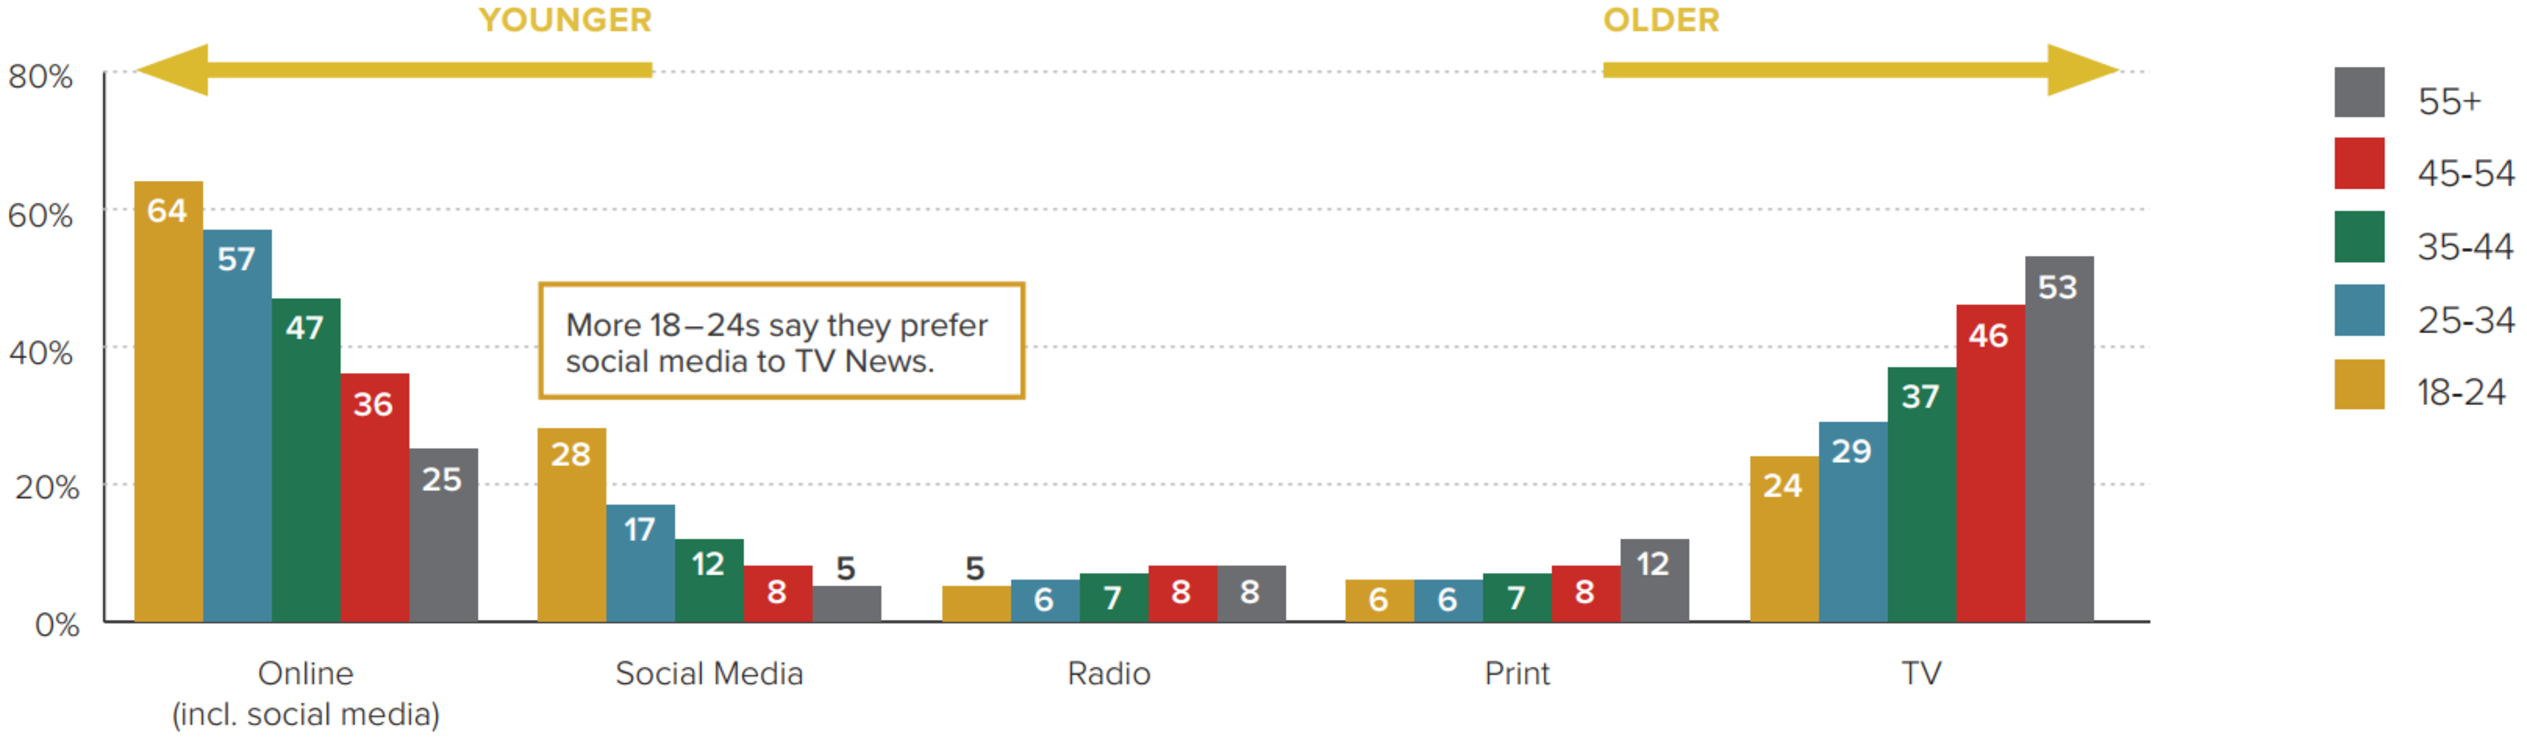
\includegraphics[width=\textwidth]{reuters-news-sources-ages}
	\caption{Main news sources split by age \cite{reuters_social_media}}
	\label{fig:reuters-news-sources-ages}
\end{figure}
% Distribution
Not only is social media more and more becoming a major distribution channel for news, it also starts delivering input for news and story creation.
This way social media has become both the source and outlet for investigative journalism.

%% Rise of the smart-phone
% Ubiquity
A smart-phone has the unique property of being a ubiquitous device that is highly mobile and extremely connectible.
Figure \ref{fig:smartphone-sales} shows that world-wide 1,4 billion smart-phones were sold to end-users last year.
And this number keeps rising.
Even or especially areas without traditional infrastructure they are ubiquitous.
\begin{figure}
	\centering
	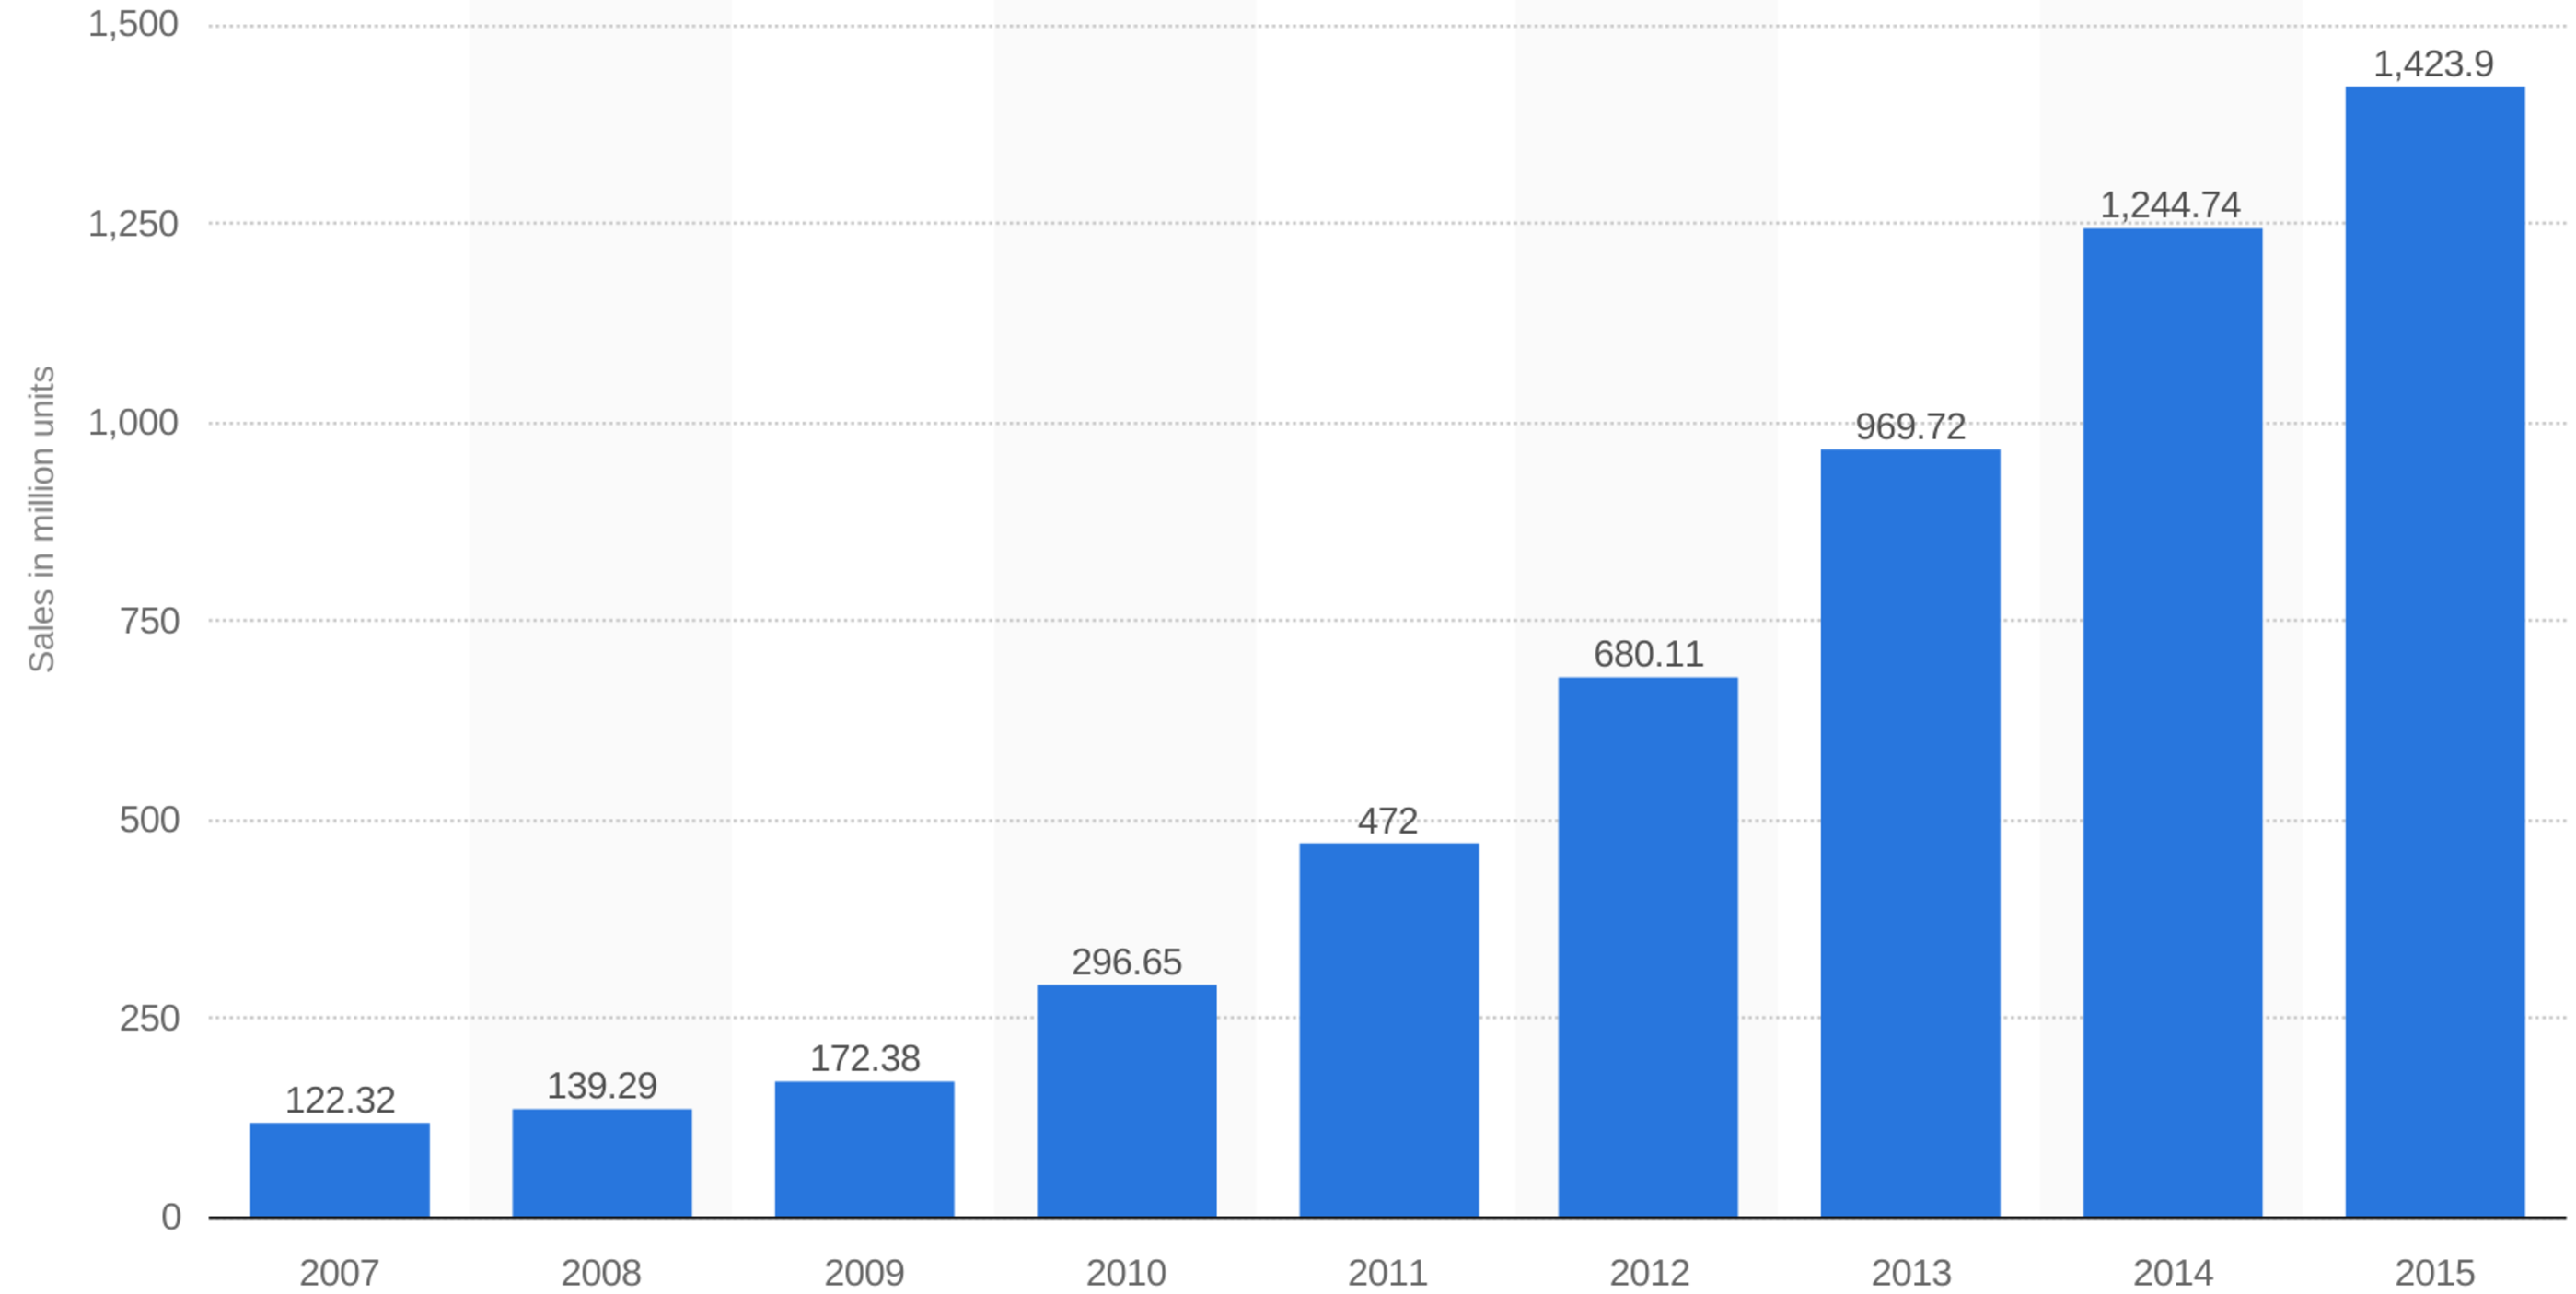
\includegraphics[width=\textwidth]{smartphone-sales}
	\caption{Number of smartphones sold to end users worldwide from 2007 to 2015 (in million units) \cite{smartphone-sales}}
	\label{fig:smartphone-sales}
\end{figure}

The capabilities and versatility of smart-phones enable it to be used for production and consumption of news and social media.
The users themselves are turning from con-sumers into pro-sumers.
% Production
% Distribution
With regards to production most smart-phones have one or more cameras to record multi-media content that can be shared immediately from the device.
Eye-witnesses often have smart-phones at hand to immediately record an event with and post it on social media.
No news desk or professional equipment is necessary to relay news directly from eye-witnesses to the masses anymore.
% Social journalism
People with camera phones can reach millions of people with multi-media in a very short timespan, becoming social journalists.
% Editorial / Journalism / Processing
The ease of reaching a global audience by an individual with a smart-phone diminishes the role of an expert curator handling incoming information.

% Consumption
Also with regard to the consumption medium mobile devices increasingly replace the role of traditional outlets like TV, newspapers and other physical media.

%% Communication during crisis
In crisis situations, like natural disaster or unrest, people need to communicate and coordinate their efforts to restore safety.
In this context the smart-phone becomes particularly important because it is often carried on person and provides connectibility.

In recent calamities people could mark themselves as safe on social media, effectively broadcasting that information to all their family and friends on social media instead of contacting them one by one or not at all due to congestion in the communication channels.

However, several natural disasters have taken out the necessary infrastructure on numerous occasions for a prolonged period of time. %katrina

Therefore we require a solution to enable social media on smart-phones that does not require infrastructure. % persistent, established ??



\chapter{Problem description}
% News & generic usage

The goal of Tribler is to become an information sharing platform / video-on-demand platform that protects the privacy of its users and is resilient to attacks while not relying on existing infrastructure.
The goal of this thesis project is to enable all Tribler functionality on mobile Android devices.


\section{Shift to social media}
% Consumption
News and media consumption is shifting from traditional outlets like TV broadcasts, newspapers and other physical media to digital media and mobile devices.
% Production
These digital mobile devices are also capable of recording multi-media content that can be directly shared from the device.
Increasingly news and media production is shifting from traditional outlets like news desks and investigative journalism to social media like Twitter, Snapchat and Facebook.
% Distribution
It is the same device that people use for consumption and producing content is capable of sharing news and multimedia.
Eye-witnesses are able to share multimedia content with others through social media.
News and information distribution is shifting from traditional media to social media.
% Editorial / Journalism / Processing
The users themselves are turning from con-sumers into pro-sumers.
No news desk or professional equipment is necessary to relay news directly from eye-witnesses to the masses anymore.
News and consumed media over social media is to a lesser and lesser degree subject to expert opinion, editorial and adversarial journalism. \cite{reuters_social_media}
% Social journalism
People with camera phones can reach 20 million people with multi-media in a very short timespan.
Social media has been a driving force in the Arab Spring.
A global dialog is possible through social media.
Large portions of the global dialog on social media is uncontrolled by traditional media or governments.


\subsection{Rise of the smart-phone}
% What advantages does a smart phone have compared to a laptop and desktop?
Given this context mobile devices are increasingly important and smart-phone in particular.
A smart-phone has the unique property of being a ubiquitous device that is highly mobile and extremely connectible.
Most smart-phones even have one or more cameras to produce multi-media content that can be shared immediately from the device.
Finally the entire world has a smart-phone.
Even or especially areas without traditional infrastructure they are ubiquitous.


\section{Communication during crisis}
% Single point of failure
With servers central to the design of typical communication networks they create a single point of failure, even in a decentralized set-up.
Several natural disasters have taken out the necessary infrastructure on numerous occasions for a prolonged period of time.
Especially in situations like these, people need to communicate and coordinate their efforts to restore safety.

In crisis situations, like natural disaster or unrest, the smart-phone becomes particularly important, exactly for the earlier mentioned properties.
Under certain conditions utilizing centralized infrastructure is undesired because of overloading the emergency communication network or physically impossible.

Social media has played a major role in recent calamities when people could mark themselves as safe, effectively broadcasting that information to all their family and friends on social media, instead of contacting them one by one or not at all due to congestion in the communication channels.


\section{Censorship}
% Single point of entry
Internet exchange (IX) infrastructures are among the central components in the inter-network architecture that are also vulnerable to monitoring, censorship and Internet kill-switches.
As such, not everyone has unrestricted access to the Internet due to censorship and surveillance.
In fact a significant part of today's Internet users is affected by these attempts to hide or distort reality. %ref
This interference directly affects the universal right to freedom of opinion and expression as stated in article 19 of the Universal Declaration of Human Rights (UDHR).

The Internet makes it easy to communicate freely on a global scale.
Connecting to it and crossing international borders on-line does not require approval of any governmental body. % wrong!
This freedom due to the absence of oversight and control allows anyone with the capability to monitor, filter, delay, or block Internet traffic at will.


\subsection{Invasion of privacy}
% Large scale monitoring

The lack of anonymity becomes a problem when the users privacy is being invaded.
Revealing personal information can be deduced from search queries for example, or associations on social platforms.
When this information can be used for targeted advertising it becomes very valuable, and creates an incentive for the parties that have access to this information to sell it to third parties.
In fact the business model of social media appears to be serving targeted advertisements to its users on behalf of third parties.
What's even worse is social media integrated into regular websites to de-anonymize and track the whereabouts of users even outside of the social media realm.
Whenever users lose control over their privacy it becomes a serious problem.

% Privacy
Pervasive monitoring of digital citizens by Internet providers on behalf of governments to enforce censorship laws raises severe privacy concerns.
Even the business model of social media companies directly conflicts with user privacy.
Targeted advertising requires the very information of high quality (accurate and current) users tend to share with their friends on-line.
When this information is shared with other parties outside of the specific social media website, possibly unknowingly to the user, it effectively becomes a privacy leak.
Subsequently users can be confronted with their information being misused in various ways beyond their control.
This lack of control over your own privacy can lead to arbitrary interference as defined in UDHR article 12. %ref, example, human rights watch, nelie kroes, etc.
Integration of social media on regular websites aggravates this problem.
Every page-view and click on social media enabled websites becomes traceable to an individual, directly benefiting the business model of targeted advertisements

% Internet censorship 2
The incentive to de-anonymize the user, not only causes a lack of privacy, but also a potential lack of freedom of expression, as it hands key information to the censor: who is expressing dissent and who is associated with this person on-line.
Cyber suppression has become a reality when you no longer can be associated with opinion-makers or foreign journalists on-line.


The sophistication of censorship techniques is pushed forward by the drive to stay ahead of attempts trying to circumvent it.
Increasingly though, Internet traffic is put under surveillance and obfuscation techniques are targeted by restrictions.


\subsection{Adversary model}
To ensure that no controlling party can exercise censorship we distribute authority over all users, creating an \emph{autonomous} system.
If all information is located in one or a few places, the parties in charge of that location will still have control over it, so we must distribute information over all users, creating a \emph{communication} system.
Then if all users want to use this system to share, order and appreciate each others information, in other words the essence of social media: social interaction, with everyone being able to interact in the same way, we need to  distribute functionality over all users, creating a \emph{cooperation} system.

% Solution
Fully distributed systems capture these characteristics.
Without any central component in the system it is no longer susceptible to censorship without everyone participating.

Decentralized can work in these situations.
Censorship and large scale monitoring is difficult in decentralized networks.
The Arab spring has shown that social media can work. \cite{Johan_2001}

Peer-to-peer communication technology is essential for a server-less distributed system.
Mobile devices typically do not require infrastructure to exchange information, like those equipped with Bluetooth or capable of ad hoc Wi-Fi.
Smart phones are ubiquitous everywhere in the world and used to access social media and retrieve information from the Internet.
Fortuitously these are also the type of mobile devices that can communicate peer-to-peer.



\section{Explore environment}
% learn about domain
% current state of technology
% what others before me have researched and accomplished

% Fragmented
Various initiatives have been started to deal with one or both of these problems. \cite{re_decentralize}
%ToDo: From re-decentralized: top projects that match/compare.

Figure \ref{fig:youbroketheinternet} shows a mapping of projects that are or have been working on that.
The fragmentation is clear from the figure and none of them provide a full solution.

%being first
%engineering perfection
%time to market
%popularity
%make a difference
%Tribler mobile vs periscope
%fully functional prototype, but poor user interface (unpolished)
%real world impact proven insufficient
%we want to change the world implicit


% Refereren aan eigen werk versplintering in oplossingen
There is no de-facto solution available on mobile platforms. \cite{literature_survey}
Previous research has shown that there is no solution that solves the problem entirely in a sustainable way.
Tribler is our attempt to solve this problem entirely in a sustainable way.
To see if it is feasible to apply it in a mobile context as described above, we need to port it.

% Previous Tribler-mobile app's
Previous attempts failed to deliver all functionality.
Maintainability issues with earlier designs were a large part of the reasons why.
We changed the architecture of Tribler for our approach.


% Contributions
By making Tribler available on mobile devices all research, with regard to the problems that Tribler tries to solve, now becomes possible on the mobile platform.

Tribler features


using UDP rather than TCP.
This privacy feature requires a lot more bandwidth of the network than without anonymity: a ratio of 13 GB for every anonymous 1 GB of data.
Since bandwidth is limited and transitory it can be beneficial to exchange unused bandwidth for a promise of bandwidth in the future, or another reward.
The research group behind Tribler is currently building a fully decentralized accounting system and open exchange market using block-chain technology with the purpose of building trust on-line and creating the Internet of Money.
% not only benefit the users thanks to an increase of available bandwidth, but more importantly  MAYBE more users, more bandwidth necessary. % Credit mining on device A to be consumed on device B.
Expanding the Tribler network would improve the usefulness of experiments on the live network for this large scale system.


\subsection{Tribler} %desktop version
% tribler and dispersy intro, what is it (read thesis independently)
%EXPLAIN what has been done to fix attack-reselience, VOD, self-organising, etc...

Tribler introduces a server-less video-sharing platform with privacy enhancing technologies and giving a Youtube-like, social media experience at the same time.
The capability of hiding your identity is greatly advantageous to the user if his or her human rights are violated, like free speech.

The server-less technique of Tribler is resistant to Internet kill-switches that are typically deployed for the purpose of censorship.

%what is the gap?
%GAP: no connection between puzzle pieces, that actually works on mobile


What is VOD?
What are the existing modules we re-use?


\section{Thesis definition}
The main question thus becomes:
How to create a \emph{self-organising} \emph{video-on-demand} platform that is \emph{attack-resilient} and can \emph{operate autonomously} on a \emph{mobile device}?

Self-organising in the sense that the platform coordinates the exchange of videos and meta-data fully automatically.

Video-on-demand in the sense that users can simply click and play videos in a streaming fashion, so without waiting for the entire video to be present on the device.

Attack-resilient in the sense that:
First: censorship does not have an effect if the majority of users does not cooperate with the censor.
Second: the privacy of users remains protected while they actively participate on the platform
Third: no network infrastructure required for viral spreading of the entire video platform.

Autonomous operation in the sense that users do not have to manage any files or configuration manually at all to be active on the platform.

Mobile device in the sense that it is low-powered and portable including the network interface and power supply.

These properties will ensure social media with resilience against Internet kill switches, natural disasters and censorship.


\chapter{Towards Tribler on mobile devices}

In the last chapter we discussed the usefulness of Tribler functionality running on desktop and server machines.
To bring that to mobile devices will give access to the usefulness of Tribler for people on the move.
Expanding the Tribler network would also improve the usefulness of experiments on the live network for this large scale system.

Properties (positive and negative) that come from these features are transferred to mobile devices, which will add their own distinct properties to the mix.


How to create a \emph{self-organising} \emph{video-on-demand} platform that is \emph{attack-resilient} and can \emph{operate autonomously} on a \emph{mobile device}?

Mobile device in the sense that it is low-powered and portable including the network interface and power supply.


% In terms of Functionality

\section{Opportunities}

What does mobile allow in addition to desktop?

Mobile devices are inherently easy to move around and very portable.
In case of a breakdown in communication infrastructure the mobile devices with wireless radio transmitters can still connect ad hoc and moved within range if necessary.

Via WiFi a device can connect to the Tribler network via existing infrastructure or other peers via ad-hoc WiFi.
Using NFC Tribler can start a Bluetooth connection and transfer the installation package peer-to-peer.
Also via NFC Tribler can exchange channel ID's to subscribe to another Tribler channel peer-to-peer.
In the future the same method can be used to exchange bootstrap peers for the Tribler network.
The peer-to-peer Bluetooth file transfer could be made much faster if the WiFi Direct would be used.


\section{Challenges}

What does working on mobile phone mean?

Mobile-devices are typically equipped with batteries to operate without a power cord.
Considering the size and weight the capacity is limited.
Smart-phone batteries usually barely hold a charge that would sustain a day of heavy usage.
Tribler could potentially drain the battery fast.
Heavy encrypted network traffic not only demand constant radio transmissions, but also CPU processing.


3 tunnels = 3x heavy
\chapter{Design and architecture}
% Intro per chapter, refer to problem definition each time, where are we now, what now (for reader)
% Why this chapter
% Paragraphs
% Conclusion of contents of this chapter
% Link to next chapter

We now present a design to address the challenges and utilize the opportunities of working on a mobile device as put forward in the previous chapter.
First in terms of functionality and other requirements, second the overall system architecture.

% now we move Tribler to mobile, so... we need these:

\section{Design principles}
Previous attempts at designing a mobile version of Tribler failed to properly separate re-usable components.
This resulted in unmaintainable code and increased difficulty in testing.
We use a top down approach to come to a high level system architecture and in determining the reusable components or the current Tribler code.
% What is the gap?
Some functionality of Tribler has been shown to work on Android before.
Our design will fill in the gap of connecting the pieces of the grand puzzle to make Tribler fully work on mobile.

% Divide and conquer
Recent refactoring of the Tribler code has divided functionality into core modules.
% Increase cohesion where possible
% Reduce coupling where possible
The purpose of this was to increase cohesion inside modules and the core, and reduce coupling between modules where possible.
This makes porting the core and individual modules easier.
% Increase re-usability where possible
Our design also attempts to maximize re-use-ability with separation of components and clearly defined interfaces.
An API between front-end and back-end is the industry standard of choice here.
% Reuse existing designs and code where possible
% What are the existing modules we re-use?
Having separated the GUI from the back-end, we can easily re-use the Tribler core and ditch the outdated wxPython GUI.
The new GUI can concentrate on Android and smart-phone user interaction.
% Keep the level of abstraction as high as possible
Many established best practices, like Google's "material design", and support libraries that abstract from platform specifics can be re-used.
% reuse of expertise
% reuse of standard designs and algorithms
% reuse of libraries of classes or procedures, of of powerful commands built into languages and operating systems
% reuse of frameworks
% reuse of complete applications
Instead of re-implementing multi-media functionality and player interface, we should re-use an existing library or preferably an entire app.
% Design for flexibility / adaptability
The flexibility of the design benefits from cohesive components with a clearly defined role.
For example: being able to swap out components like the GUI makes Tribler much more adaptable to various mobile devices that may or may not have a display.
The configuration of Tribler core is stored separately from the data and can be altered externally by users since it is saved in a human readable form.
% Anticipate obsolescence
% niet echt iets mee gedaan

% Design for portability
All functionality of Tribler must be packaged in a single installable container.
% Design for testability
The GUI must be able to be tested separately from the back-end and vice-versa.
Also the API must be able to be tested independently and be clearly documented for other developers.

% Design defensively
All Android intents should be explicit. \cite{paper Analysing inter-application communication in Android}
Expose / Export only Android activities and services that should be public

% Availability and resilience
A distinction must be made between user input error and internal exceptions.
The user must be given a chance to correct the input without starting over.
If Tribler crashes it should resume normal operation by just restarting it and optionally ask the user to do so.
% Internationalization
The GUI should support other languages to be added without changing source code.
% Resource usage
The separation of front-end and back-end should not lead to resources being loaded into memory twice or anything of that matter.
% Usability
Make use of universally recognizable icons that are native to the platform UI.
The responsiveness of the GUI must not be significantly impacted by the amount of data presented on screen.
The responsiveness of the GUI must also not be significantly impacted by the amount of computational work, or otherwise, done in the background.


\section{Functional requirements}
% Functional level
% Function design
%Product design involves determining the objectives of the system. Central questions in this process are “what is feasible?”, “what is required?” and “what functions need to be fulfilled by the system?” It is a strategic decision process and it will be termed the function design 
%Function design distinguishes between innovation and improvement. Improvement usually only concerns the reorganisation or reengineering of an existing system, which implies a rearrangement of existing functions or a different interpretation of these functions. Innovation concerns the extension, reduction or modification of functions due to the introduction of new technology, resources and/or organisation.

inputs, commands and conditions
outputs, conditions
store, reuse data, backup
computations
timing and synchronization


Functional requirements

Live production (screenshots) and dissemination
Record video
Create My Channel
Add to My Channel
Search results

MultiChain

Start quickly / delay

REST HTTP JSON API

GUI

Nosetests CI


All functionality of Tribler must be usable directly from the mobile device, without the need or support for any other external device.

Because of the ubiquity of smart-phones with built-in camera one is always at hand and ready to record.
Such mobile devices are much more manageable than for example laptops with built-in camera that Tribler has been capable of running on in the past.
No opportunity has to be missed due to hassle of getting a dedicated camera and transferring the recording to a connectible device afterwards.
Therefore the camera built-in the mobile device should be used to record video or photographs with Tribler.
The usability of Tribler as a content generating tool is greatly improved by this. 

Publishing content should be one simple step for the user to perform, especially right after creating new content.
Every user must be able create his/her own channel in Tribler to publish their content, just like channels in YouTube, directly from the mobile device.
Newly discovered channels and content may be added to the GUI without user interaction.

To easily share your own channel with others the id could be transferred via NFC from device to device.
With just one-click-confirmation it should be send, and the receiving device must then be able to subscribe to this channel and start discovering the contents automatically right away.
Because this may require both devices having Tribler installed, it also must be able to share the installation package via Bluetooth or WiFi without any prerequisites on the receiving device.

Self-created content must be stored on the internal memory and processed automatically on the mobile device itself in order to avoid dependency any external processing unit.
This includes the creation of .torrent files required to share content via the bit-torrent protocol.



impliceert: gewoon opschrijven: 2 processes means communication: impliceert API

%TODO: kijk naar wat in DRAFT staat, dat zijn key dingen



\section{Non-functional requirements}


\subsection{Quality requirements}


All processing tasks should be performed in the background, so as to allow the user to continue working with Tribler or otherwise, while indicating about ongoing processing.
The GUI must be responsive to the users' input at all times, even if the amount of data shown on screen is very large.

If an error occurs that is recoverable the app should automatically retry or ask the user to correct the input if applicable.

To keep the project maintainable the entire build tool-chain must be integrated in the continuous integration and build server of Tribler.
All existing tests should also be performed on Android, with modifications for platform specific tests.
Also all unit tests and integration tests must cover as much code as possible and should be executed on every build.


responsivitity through separation of front and backend


non-bloated

alleen key dingen hiervan:

response time
throughput
resource usage
reliability
availability
recover from failure
maintainability and enhancement
re-usability

\subsection{Platform requirements}

computing platform: min. system specs and features, api level
technology to be used: programming language, db

The minimum API level of Android should support WiFi, Bluetooth and NFC features.



\subsection{Process requirements}

development process / methodology
cost
delivery date




(instant) search





\section{System architecture}
% Design level


\begin{figure}[h]
	\centering
	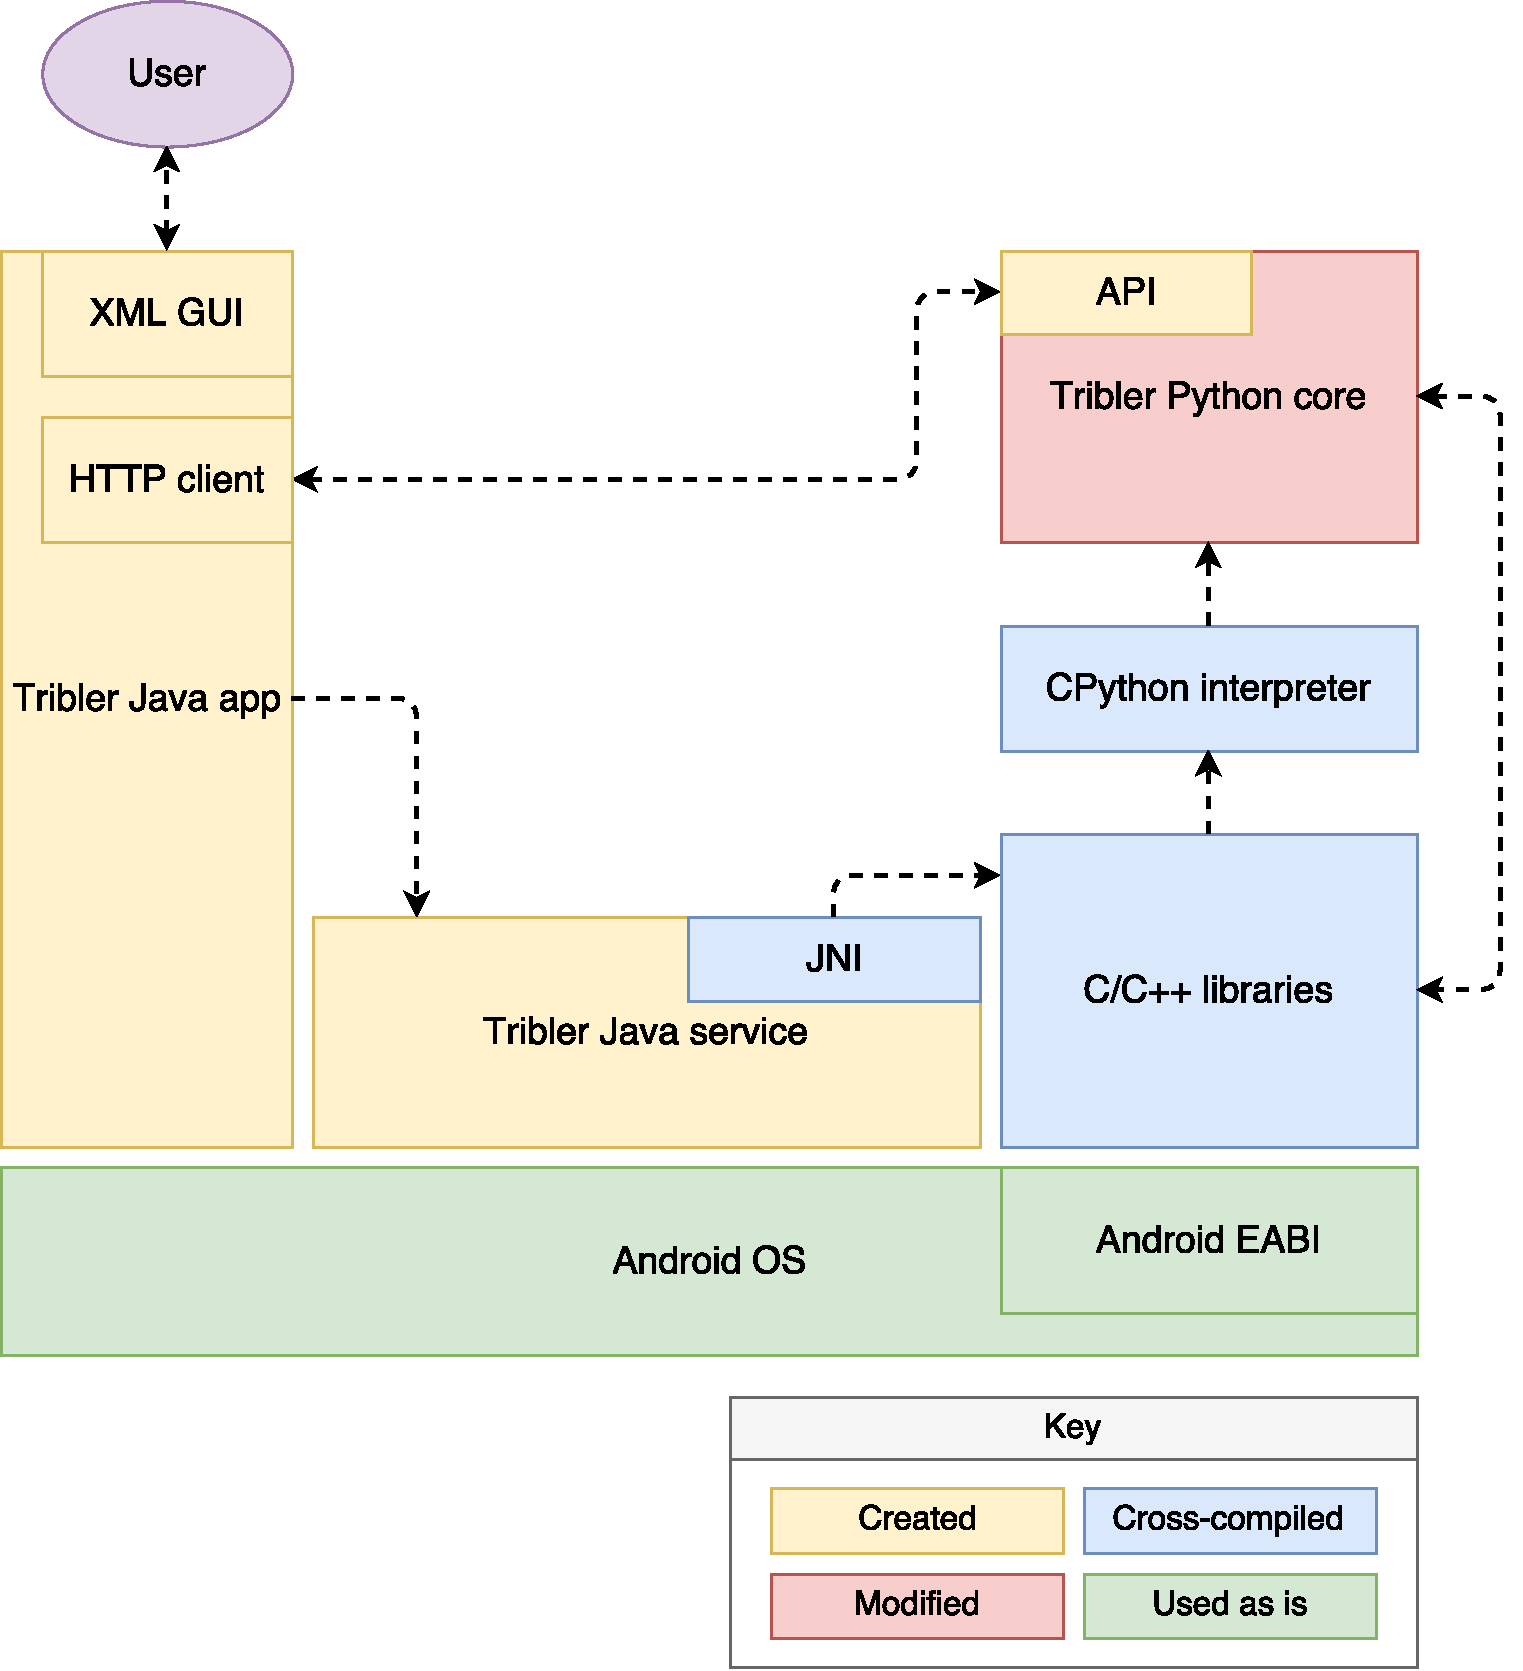
\includegraphics[width=\textwidth]{system_architecture}
	\caption{System architecture}
	\label{fig:system_architecture}
\end{figure}


Previous attempts at creating an Android version of Tribler failed with regards to maintainability.
Poor separation of front-end and back-end meant re-use of the core modules was hard to maintain.
The new architecture clearly separates tasks of the GUI and background operations.



\chapter{Implementation}

\section{Develop and organize} %implementation
%low prio


Verkopen: app build with reactive programming paradigm, Rx founded by TU Delft professor

code example
modular functional programming



\section{Tool-chain architecture}


we transfered the first generation bash script into a more involved python tool chain ecosystem
the p4a project accepted our first contribution the same day
our approach for this .. we focused on the low hanging fruit first to benefit from the learning effect
the first task consisted of porting the python bindings for 15 - 30+ commonly used libraries to Android [recipe example code block]

\subsection{Python-for-android}
Open source project p4a uses python toolchain with bootstraps, recipes, ant, make, Android SDK (aapt), Android NDK, zipalign, ..., setuptools, ...

\subsection{Gradle experimental}
Use Android SDK, jni, Android NDK, ...


\section{System architecture}
table of lines of code
modules app

\subsection{Python on Android}
Open source project Python-for-Android is capable of running python code.

no shell acces from Popen() means only single binaries instead of normal commands

\emph{My contributions:}
\begin{itemize}
	\item add service only bootstrap with templates
	\item recipe (missing) for all dependencies
	\item bug fixes in build tool chain
	\item service interface binder
\end{itemize}


\subsection{Rest API}

\emph{My contributions:}
\begin{itemize}
	\item create channel
	\item create torrent
	\item add torrent to channel
	\item async download and add torrent to channel from url and magnet links
	\item remote shutdown
\end{itemize}

\subsection{Common python core}

\emph{My contributions:}
\begin{itemize}
	\item correct paths for Android
	\item setup.py rewrite
	\item improve error handling in test runner
	\item various threading bug fixes
\end{itemize}


\subsection{Native Android GUI}
Gui for common core back-end and rest api in between.

\emph{My contributions:}
\begin{itemize}
	\item Native service wrapper for Python process
	\item GUI:
	\item create own channel
	\item record video
	\item create torrent file
	\item add torrent to own channel
	\item search torrents and channels
	\item voice search integration
	\item view channel contents
	\item download torrent
	\item launch video viewer
	\item mark and un-mark channel as favorite
\end{itemize}



\chapter{Performance analysis}\label{ch:results}
% Validation: Are we building the right system?
% Verification: Are we building the system right?
To analyze how feasible is it to run all Tribler functionality on mobile devices, we measure several performance characteristics relevant to the functional and non-functional requirements in Chapter \ref{ch:design}.
We take several measurements on different devices to quantify the performance and resource usage in the context of the scenario in the problem description in Chapter \ref{ch:problem_desc}.
The results will indicate the state of the art, before any optimization, in functionality of Tribler on mobile devices as described in Chapter \ref{ch:tribler}.
From the results, possible angles for optimization will emerge and further described in Chapter \ref{ch:conclusions}.
The results also show that all requirements have been met.

% Rationale
% Metrics
% Expected / desired results
% Setup
% Results
% Conclusions

\section{Content discovery}\label{sec:content_discovery}
%TODO: 2 subvragen: creation "req.X" (8) & adding "req.Y" (8) & discovery "req.Z" (15)
% laat zien dat linair verband aannemelijk is voor creation & adding
%TODO: acquisitie van data uitbreiden
%meta info does not scale with content size
%TODO: remove times from schematic scenario figure
% Rationale
New content is generated on the device, like for example a video that has been recorded.
Before anyone can view that content it has to be added to a channel and discovered by other devices.
% Metrics
We measure the amount of time it takes for other devices, which are subscribed to the channel, to discover new content.
We also measure the amount of time it takes for content to be added to a channel in the form of a torrent.
The amount of time it takes for a torrent to be created is relative to the size of the content.
Therefore these measurements are normalized to a file of 1 MB.
% Expected / desired results
Depending on the random walk in the channel's community content can be discovered either very quickly or after a while due to property of eventual consistency.
\begin{figure}[H]
	\centering
	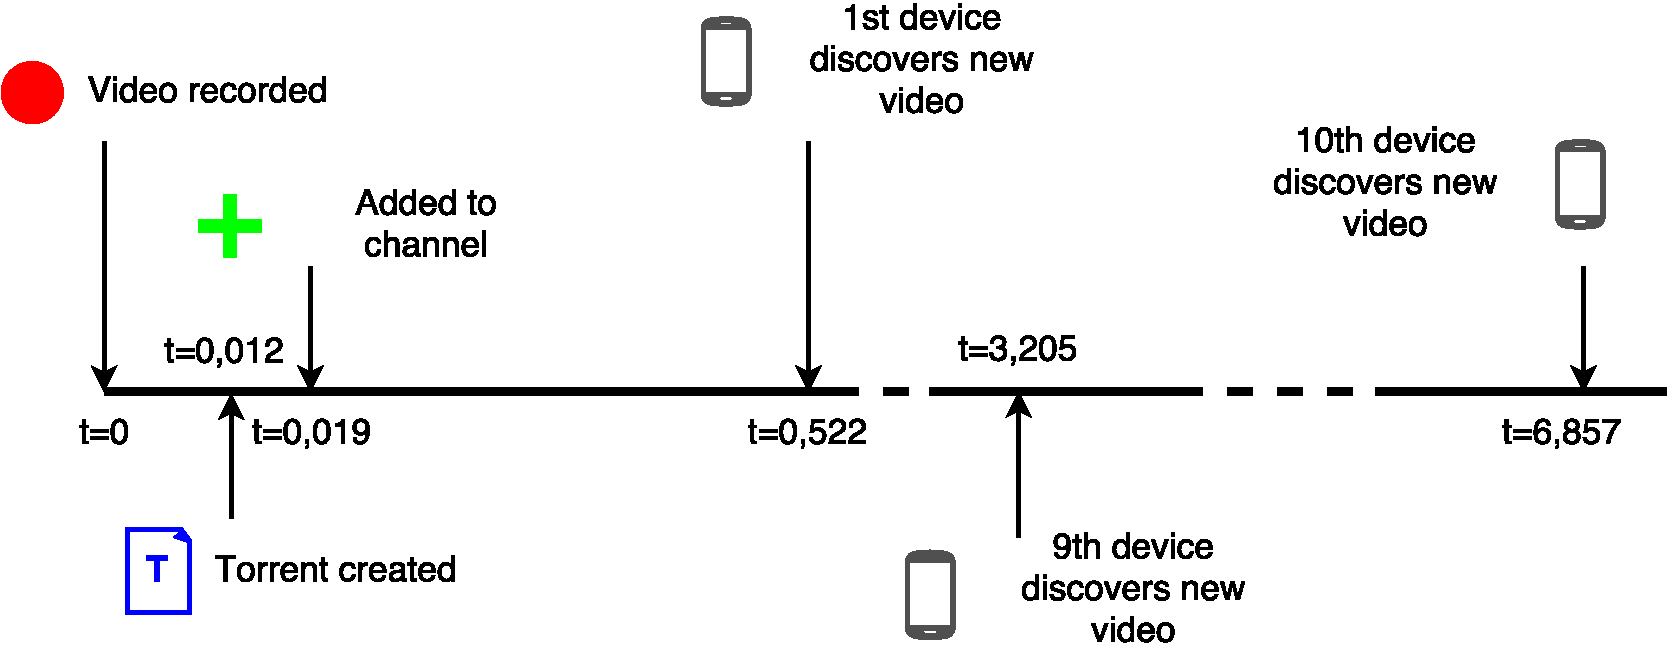
\includegraphics[width=\textwidth]{content_dissemination}
	\caption{Sequence of events when a video is recorded and distributed.}
	\label{fig:content_dissemination}
\end{figure}
% Setup
Figure \ref{fig:phones_2} shows the experimental setup with various smart-phones and one tablet.
Each device is connected to the same wireless network and within 1 to 2 meters distance from the same access point.
Different versions of Android OS are installed, ranging from 4.3 to 7.1, and some run a CyanogenMod.
Each device is installed with the same version of Tribler and the same database, containing up to date information about existing channels and their content.
This database was gathered in the days before this experiment and installed manually.
On one device, a Nexus 6, from now on referred to as the source, a new channel is created to which the other 13 devices subscribe via NFC.
Then, repeatedly a new video is recorded and added to that channel by the source.
The new videos are discovered, and the event logged, by each device individually.
All devices devices are synced with NTP to be able to have a common timeline for this experiment.

\begin{figure}[H]
	\centering
	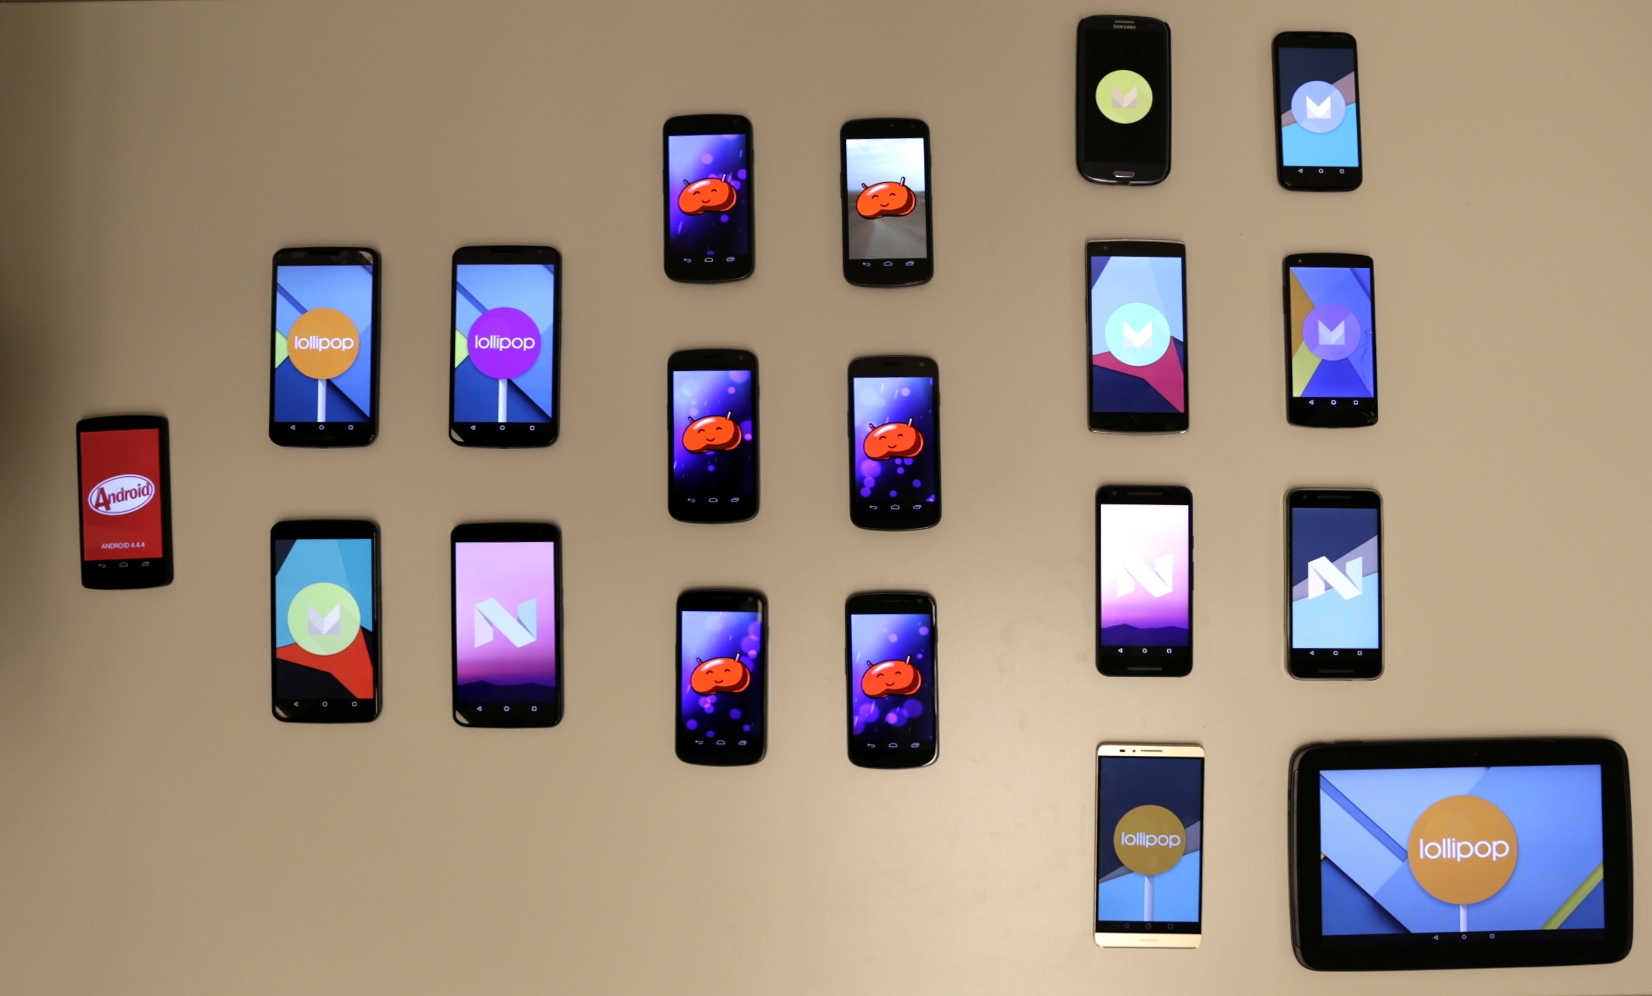
\includegraphics[width=\textwidth]{phones_2}
	\caption{Experimental setup with various smart-phones and one tablet, all showing the About Android screen.}
	\label{fig:phones_2}
\end{figure}

\begin{minipage}{.35\textwidth}
\begin{table}[H]
	\begin{tabular}{l | l} \hline
		Laptop & Dell Latitude E6520 \\ \hline \hline
		CPU & i7-2760QM @ 2.4GHz \\ \hline
		RAM & 8 GB @ 1333 MHz \\ \hline %% NT4GC64B8HG0NS-CG
		SSD & 80GB X25-M \\ \hline %% SSDSA2M080G2GC
	\end{tabular}
	\caption{Hardware specifications of the laptop used in the Multichain and API measurements.}
	\label{table:specs_laptop}
\end{table}
\end{minipage}
~~~~~~~~~~~~~~~
\begin{minipage}{.69\textwidth}
\begin{table}[H]
	\begin{tabular}{l | l} \hline
		Amount & Device \\ \hline \hline
		6 & Galaxy Nexus \\ \hline
		4 & Nexus 6 \\ \hline
		1 & Nexus 5, Nexus 10, Galaxy S3, OnePlus One \\ \hline
	\end{tabular}
	\caption{Devices used in the content discovery experiment.\\}
	\label{table:devices}
\end{table}
\end{minipage}

% Results
\begin{figure}[H]
	\centering % trim={<left> <lower> <right> <upper>}
	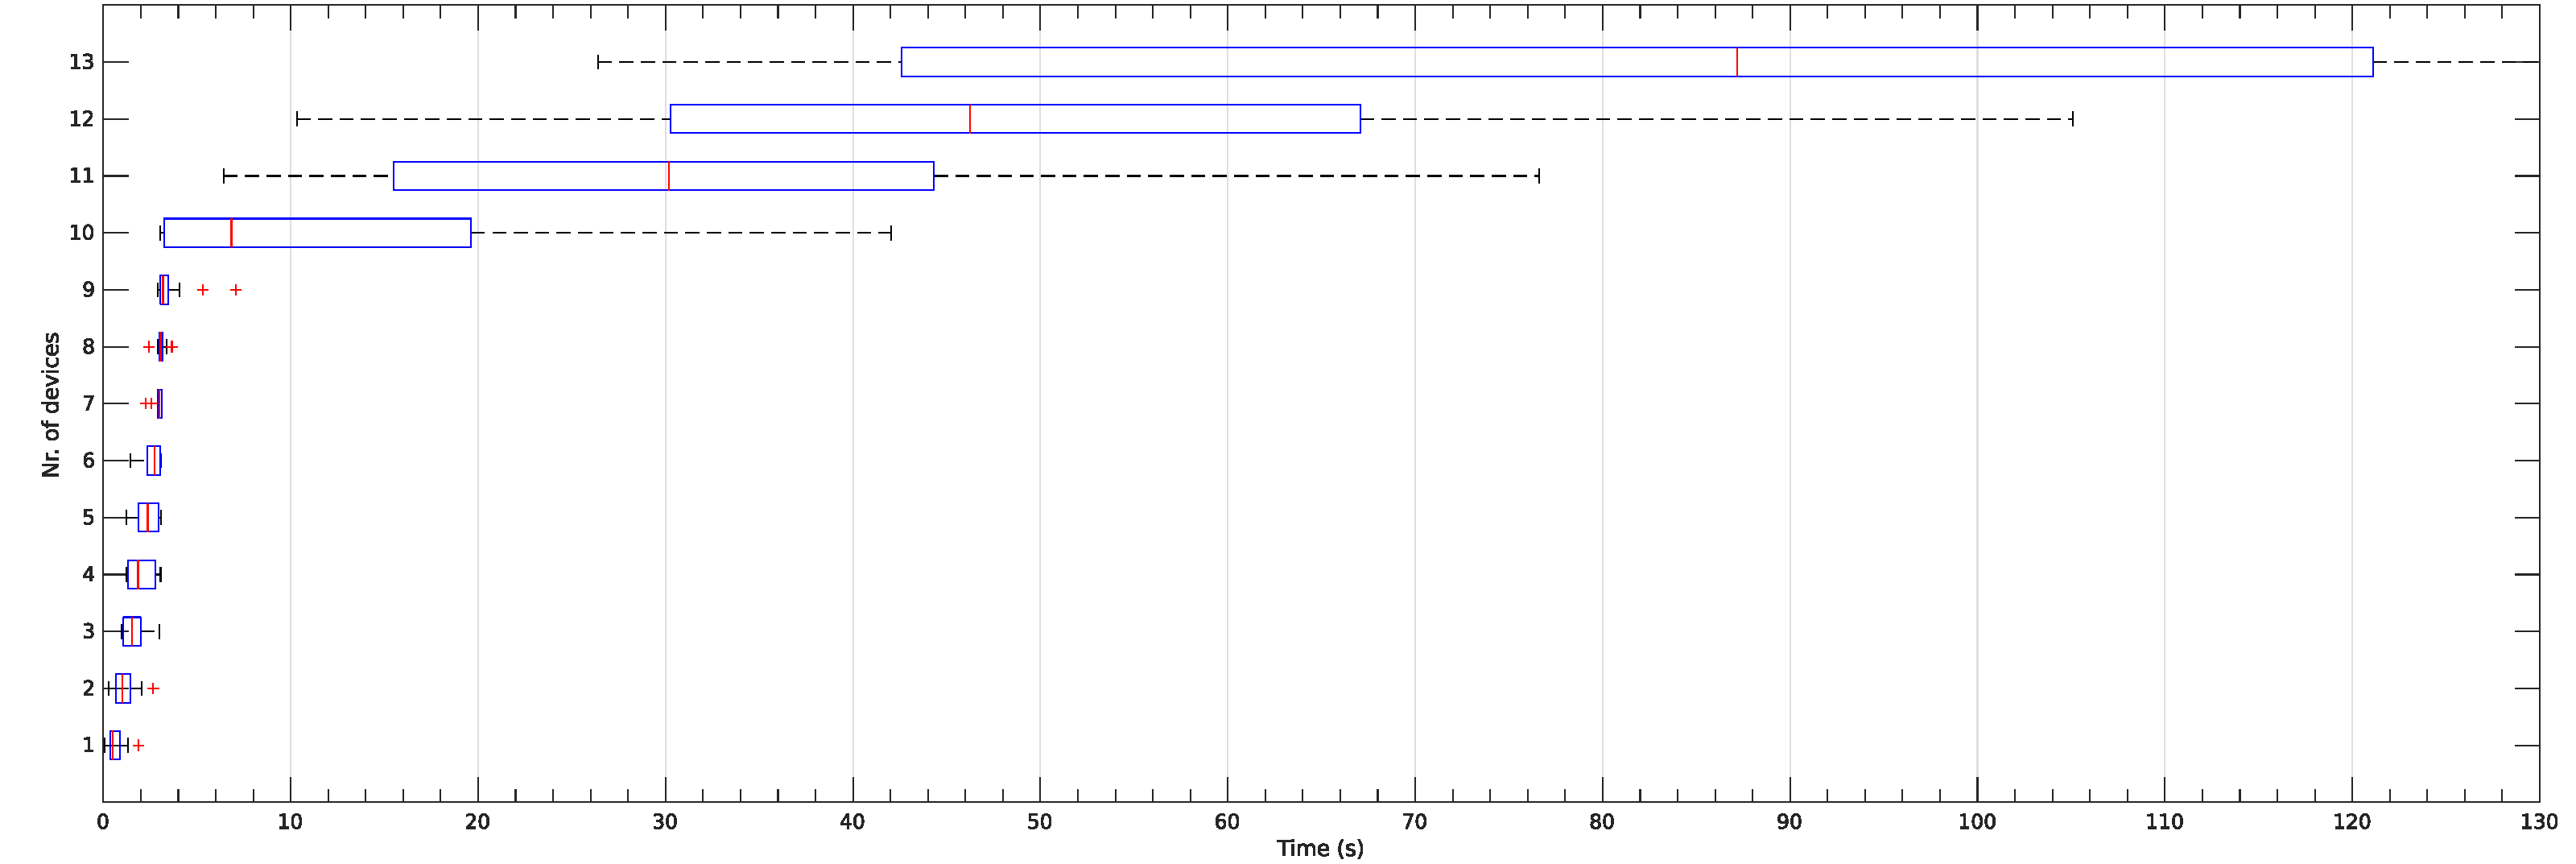
\includegraphics[trim={0.9cm 0 0 0},clip,width=\textwidth]{boxplot-nrofdevices-130}
	\caption{Elapsed time from adding new content to a channel and it being discovered by subscribed peers.}
	\label{fig:boxplot-nr.of.devices-130}
\end{figure}
Figure \ref{fig:boxplot-nr.of.devices-130} shows the amount of time it takes a number of devices to discover new content on a subscribed channel.
The results show that within 4 seconds 9 devices have discovered the new content.
From the 10th device and beyond an increase in discovery time is noticeable.
% Conclusions
This could be explained by the fact that only 10 peers are connected at the a time.
Much more peers are needed to give an accurate representation in terms of scalability.
What can be concluded from this experiment is that on the same local network the first device discovers the new content in less than 2 seconds.
From the 10th device onwards the dissemination slows down.


\section{Multichain performance}\label{sec:multichain_perf}
% Rationale
Multichain is the new accounting system of Tribler.
This feature is central to the concept of trust in the Tribler network and is very important for the future as other functionality will be built upon it.
If mobile devices are to become full-fletched nodes on the network they must support this feature.
With Multichain any peer registers the bandwidth it exchanges with other peers.
It aggregates these exchanges in blocks and signs them like a receipt and sends that to the other party to sign as well.
These blocks are linked in a block-chain to foil attempts of cheating the system.

Multichain is explicitly designed to not use a global state.
Syncing a global state is less scalable in terms of storage and network bandwidth.

% Metrics
The creation and signing of these blocks is measured to determine if it scales well.
Multichain signs a block every 10 minutes, meaning our experiment of generating 25.000 blocks represent about half a year (173,6 days) of continuous effort.
% Expected / desired results
The database containing these blocks will grow over time, but should not slow down too much because of it.
% Setup
Measurements were taken on six different devices on multiple moments during development.
% Results
Figure \ref{fig:multichain_25} show the performance graphs of every measurement.
\begin{figure}[H]
	\centering
	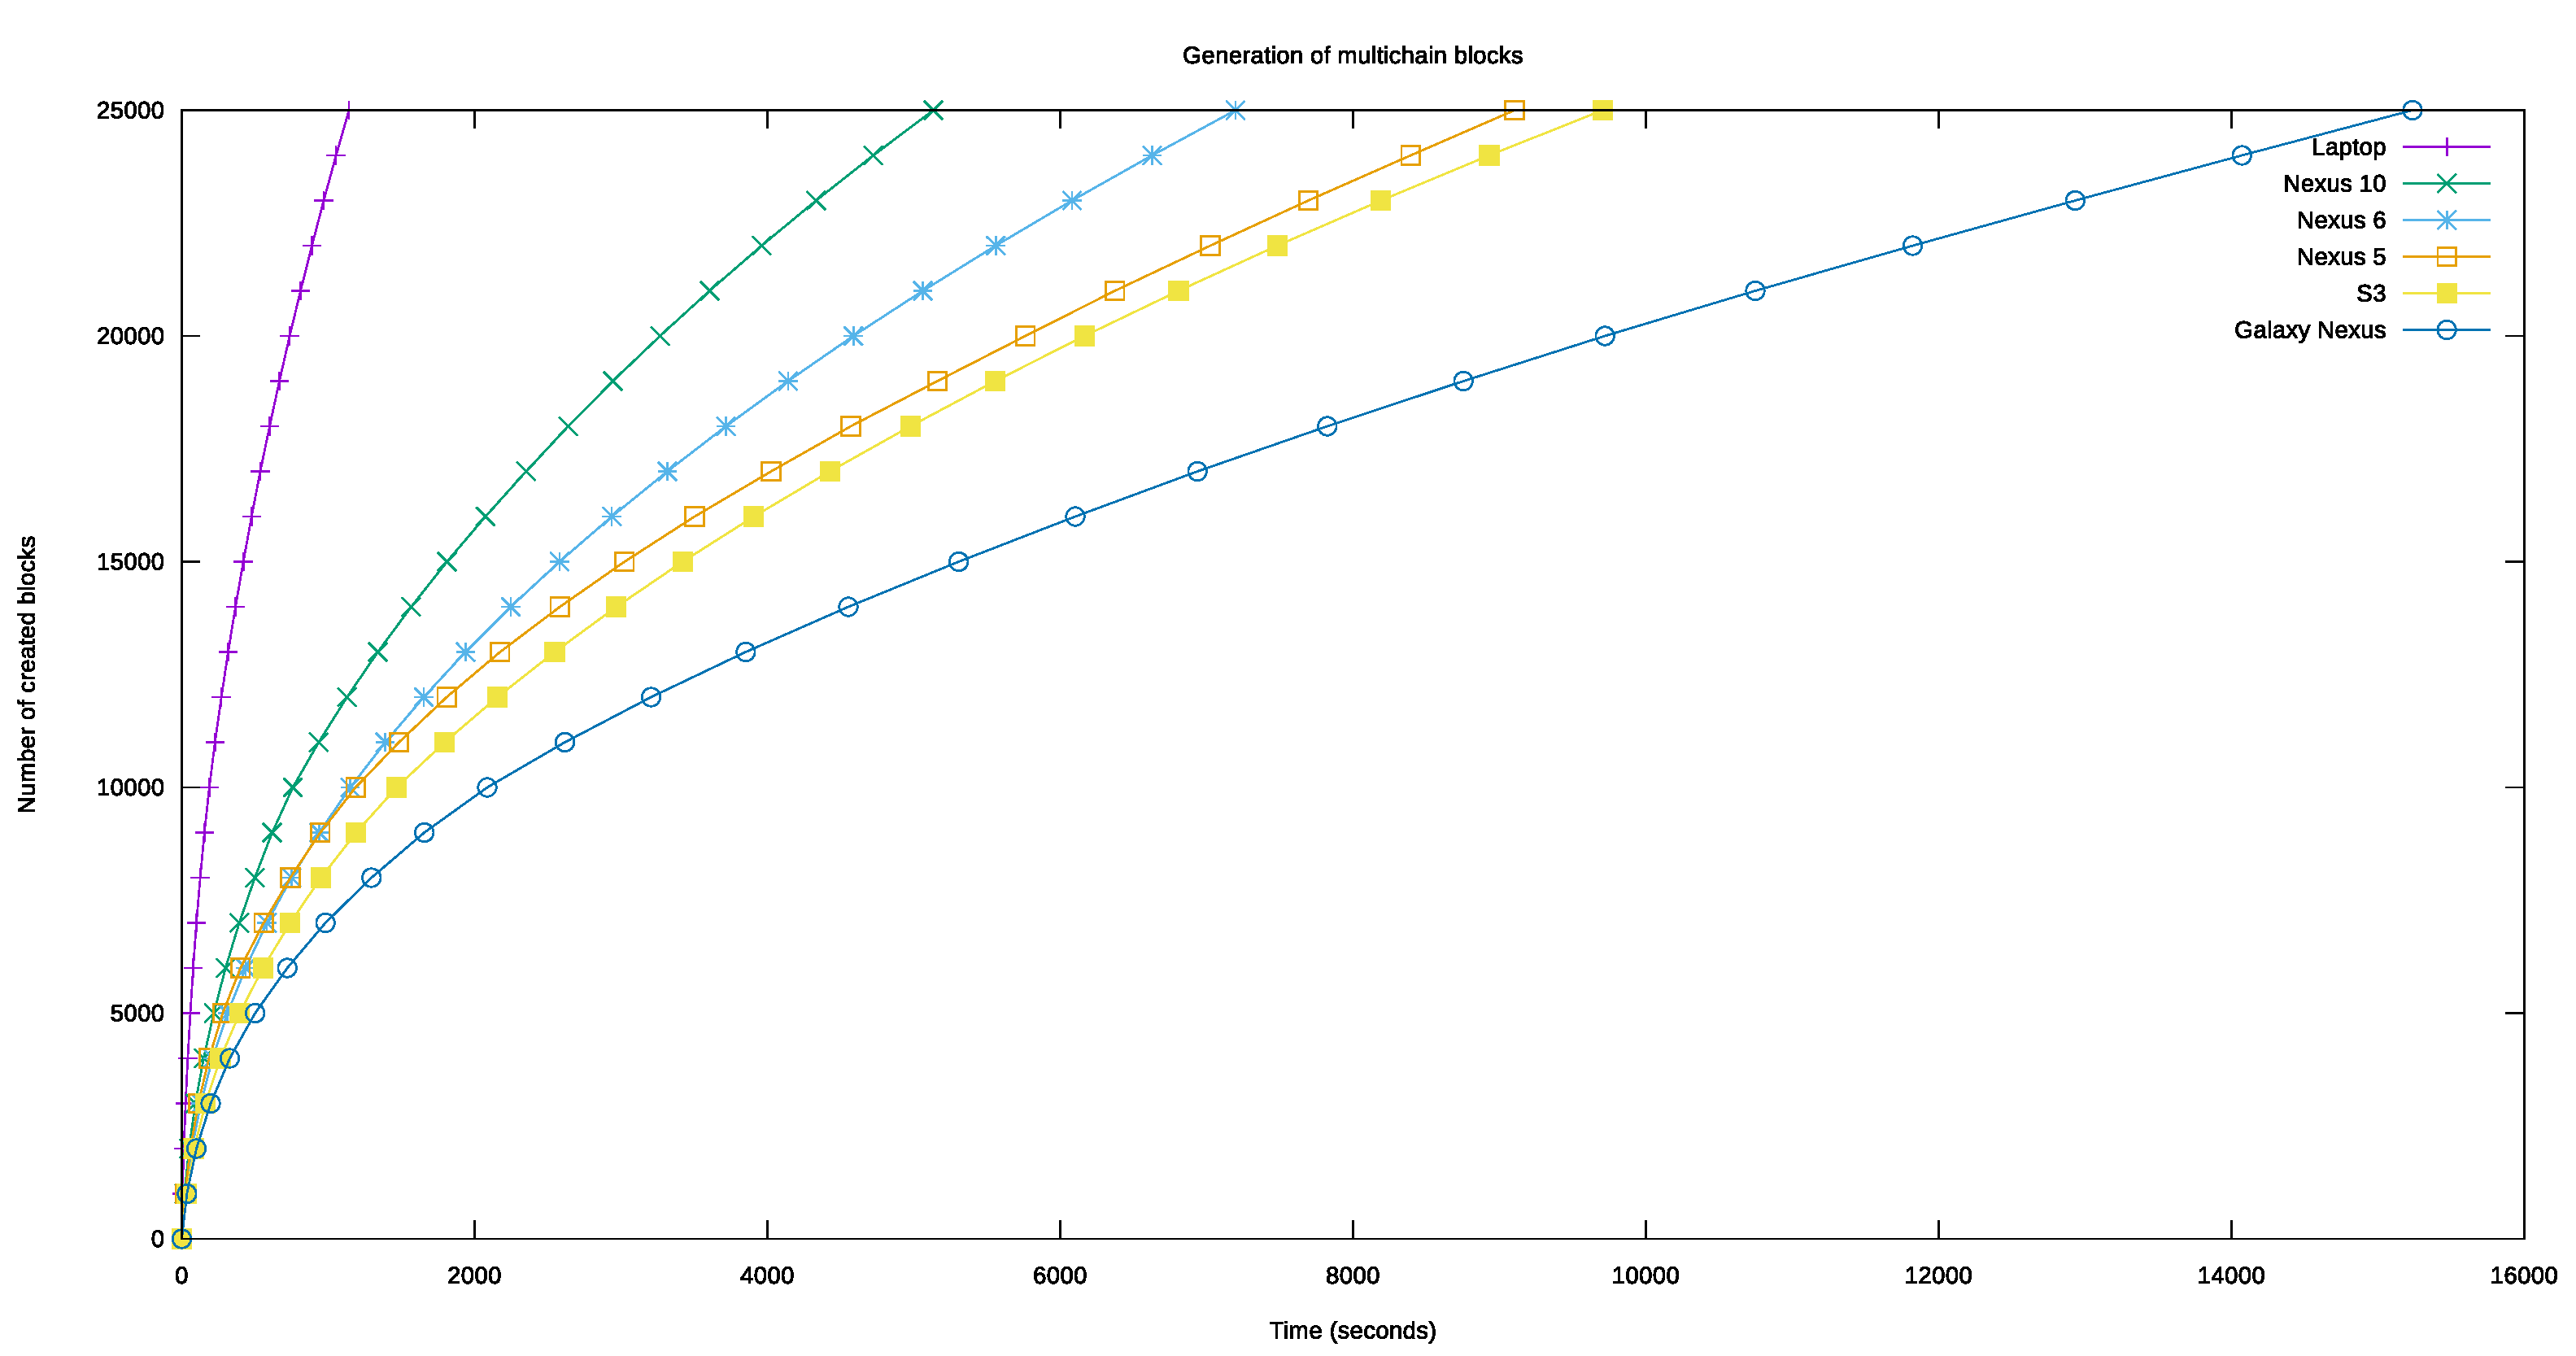
\includegraphics[width=\textwidth]{multichain_scale_2599_25k}
	\caption{Creating and signing of 25.000 blocks between two peers}
	\label{fig:multichain_25}
\end{figure}
Clearly visible from the graphs is that Multichain does not scale linearly on any device.
They also show that mobile devices are at least a factor of two slower than an ordinary laptop and scale worse.
% Conclusions
Due to the nature of block-chain every new block needs to contain the hash value of the previous block.
If a database lookup is needed for this and the database is growing, that can explain the non-linear course of the graph.
This can be easily resolved by keeping the last hash value for currently connected peers in memory.
However this is an indication that creating blocks by the thousands is an IO bound process, rather than CPU bound.
Finally, if mobile devices are to be full-fletched nodes on the Tribler network, they should not slow down significantly more than any other ordinary laptop, besides being slower in the first place.
Hardware acceleration could close this gap without sacrificing battery life too much.
Because mobile devices are a bit behind on the technology curve with respect to desktop computers it is probable that the gap becomes smaller over the coming years.
The capacity to store enough Multichain blocks to audit past exchanges should also be on par.
If not, other more powerful nodes could be queried to supply the necessary history about a peer, that requests your bandwidth, to verify if that peer is trustworthy.


\section{Startup time}\label{sec:startup_time}
%TODO previous chapter: implementation architecture startup sequence nice design, how does it perform?
% when is gui ready for real? do not say gui is response blabla because we do not measure.

% Rationale
Key to user retention is a fast startup time.
Therefore the service starts up in the background, separately from the GUI.
This way at the GUI is responsive to user input while the service may still be loading.
One of the design objectives for separating the front-end from the back-end was responsiveness.
However before any task can be executed by the service it needs to be actually started.
% Metrics
To measure the startup time we register the time of launching the app and the moment the Tribler-started-event occurs.
This event is sent over the API event-stream and signifies that Tribler is fully started and ready to accept all incoming requests.
% Expected / desired results
We expect consistent loading times because right after starting we shut Tribler down again.
% Setup
%TODO consistency within device
%consistency over different devices, explain
To get a good idea of how the user experience may differ we measure the startup time 10 times on 5 different devices.
The app is launched with Android Debug Bridge (adb) from a laptop and the Tribler-started-event is read from logcat over adb and timed on the same laptop so they use the same clock.
% Results
\begin{figure}[H]
	\centering % trim={<left> <lower> <right> <upper>}
	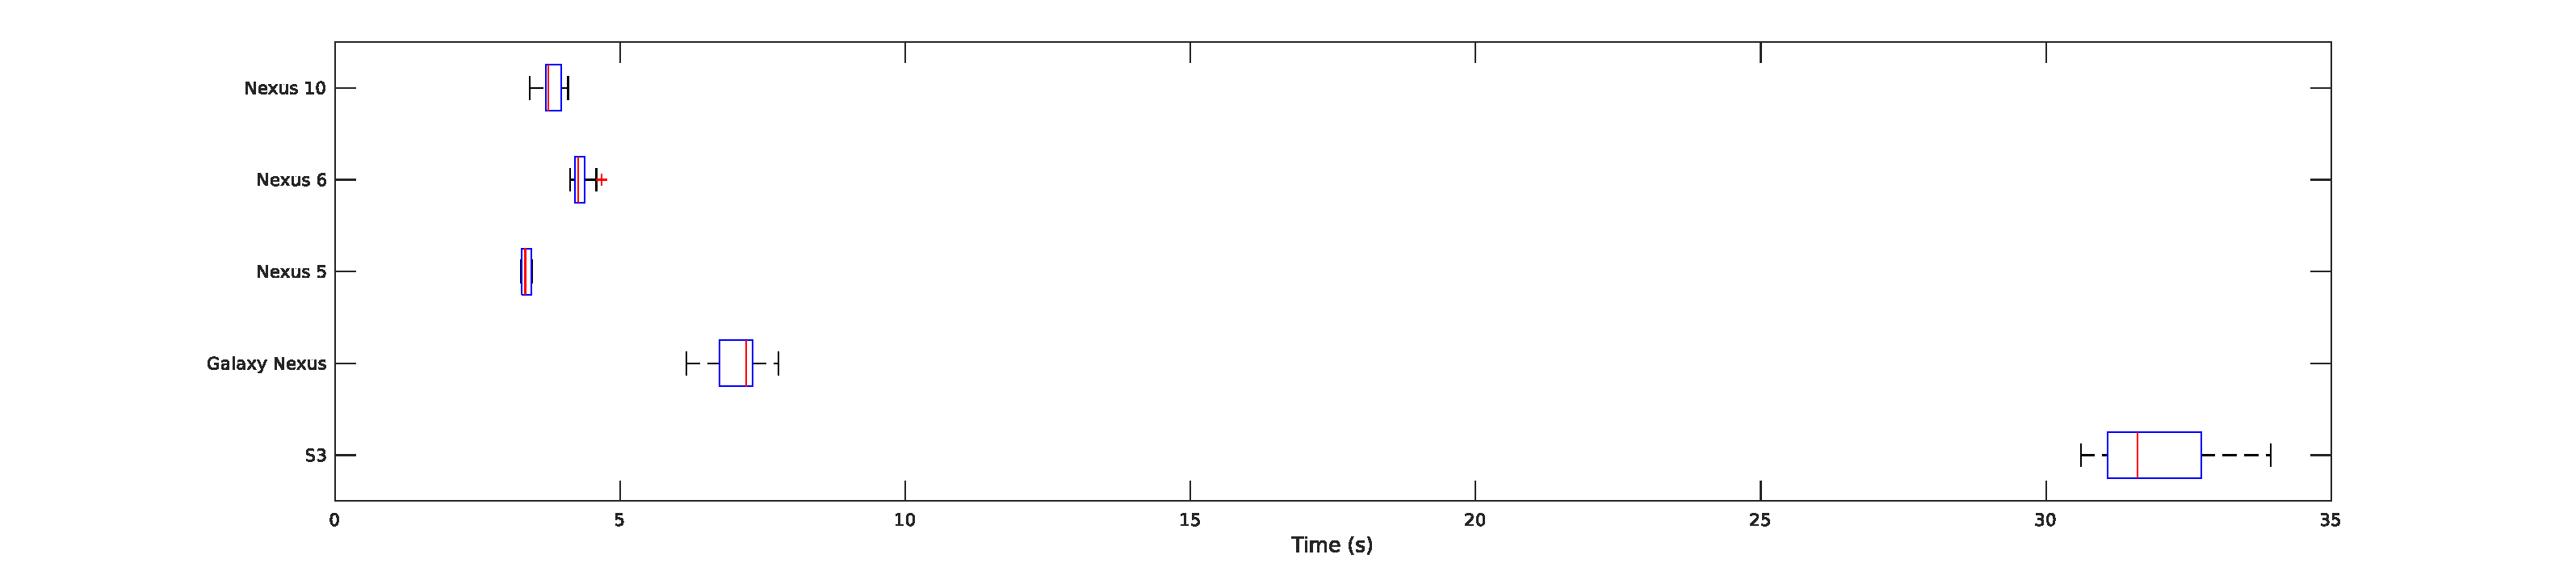
\includegraphics[trim={4cm 0cm 4cm 0cm},clip,width=\textwidth]{boxplot-startup}
	\caption{Startup times per device}
	\label{fig:boxplot-startup}
\end{figure}
Table \ref{table:startup_time} shows the statistics per device.
\begin{table}
	\begin{tabular}{l | *{5}{r}} \hline
		Device & N & Avg. (s) & Min. (s) & Max. (s) & s (s) \\ \hline \hline
		Nexus 10        & 10 & 3.781 & 3.416 & 4.085 & 0.211 \\ \hline
		Nexus 6          & 10 & 4.319 & 4.124 & 4.670 & 0.179 \\ \hline
		Nexus 5          & 10 & 3.353 & 3.273 & 3.459 & 0.081 \\ \hline
		Galaxy Nexus & 10 & 7.086 & 6.161 & 7.772 & 0.454 \\ \hline
		S3                   & 10 & 31.935 & 30.616 & 33.940 & 1.116 \\ \hline
	\end{tabular}
	\caption{???}
	\label{table:startup_time}
\end{table}
The results show a very small sample standard deviation and a very low startup time.
The S3 is performing worse than may be expected judging from the results of the other devices.
% Conclusions
The reason for that may be that this phone was not wiped and given a fresh install of Android.
That could mean that other applications installed on a device could significantly impact the performance of Tribler.
The sample standard deviation is relatively small though, which contradicts this hypothesis.
This should be investigated further, including if anything can be done on the part of Tribler.


\section{Content creation}\label{sec:content_creation}
%TODO grote scenario
% Rationale
How quick one can create content and distribute it depends not only on the discovery time, as measured in Section \ref{sec:content_discovery}, but firstly on the speed of the torrent creation process.
% Metrics
% Expected / desired results
% Setup
The setup for this measurement is exactly the same as in Section \ref{sec:content_discovery} with one phone creating the torrent file of the video content.
% Results
Figure \ref{fig:torrent-create-scatterplot} shows the relation between the size of the content and the time required to create a torrent file for it.
\begin{figure}[H]
	\centering % trim={<left> <lower> <right> <upper>}
	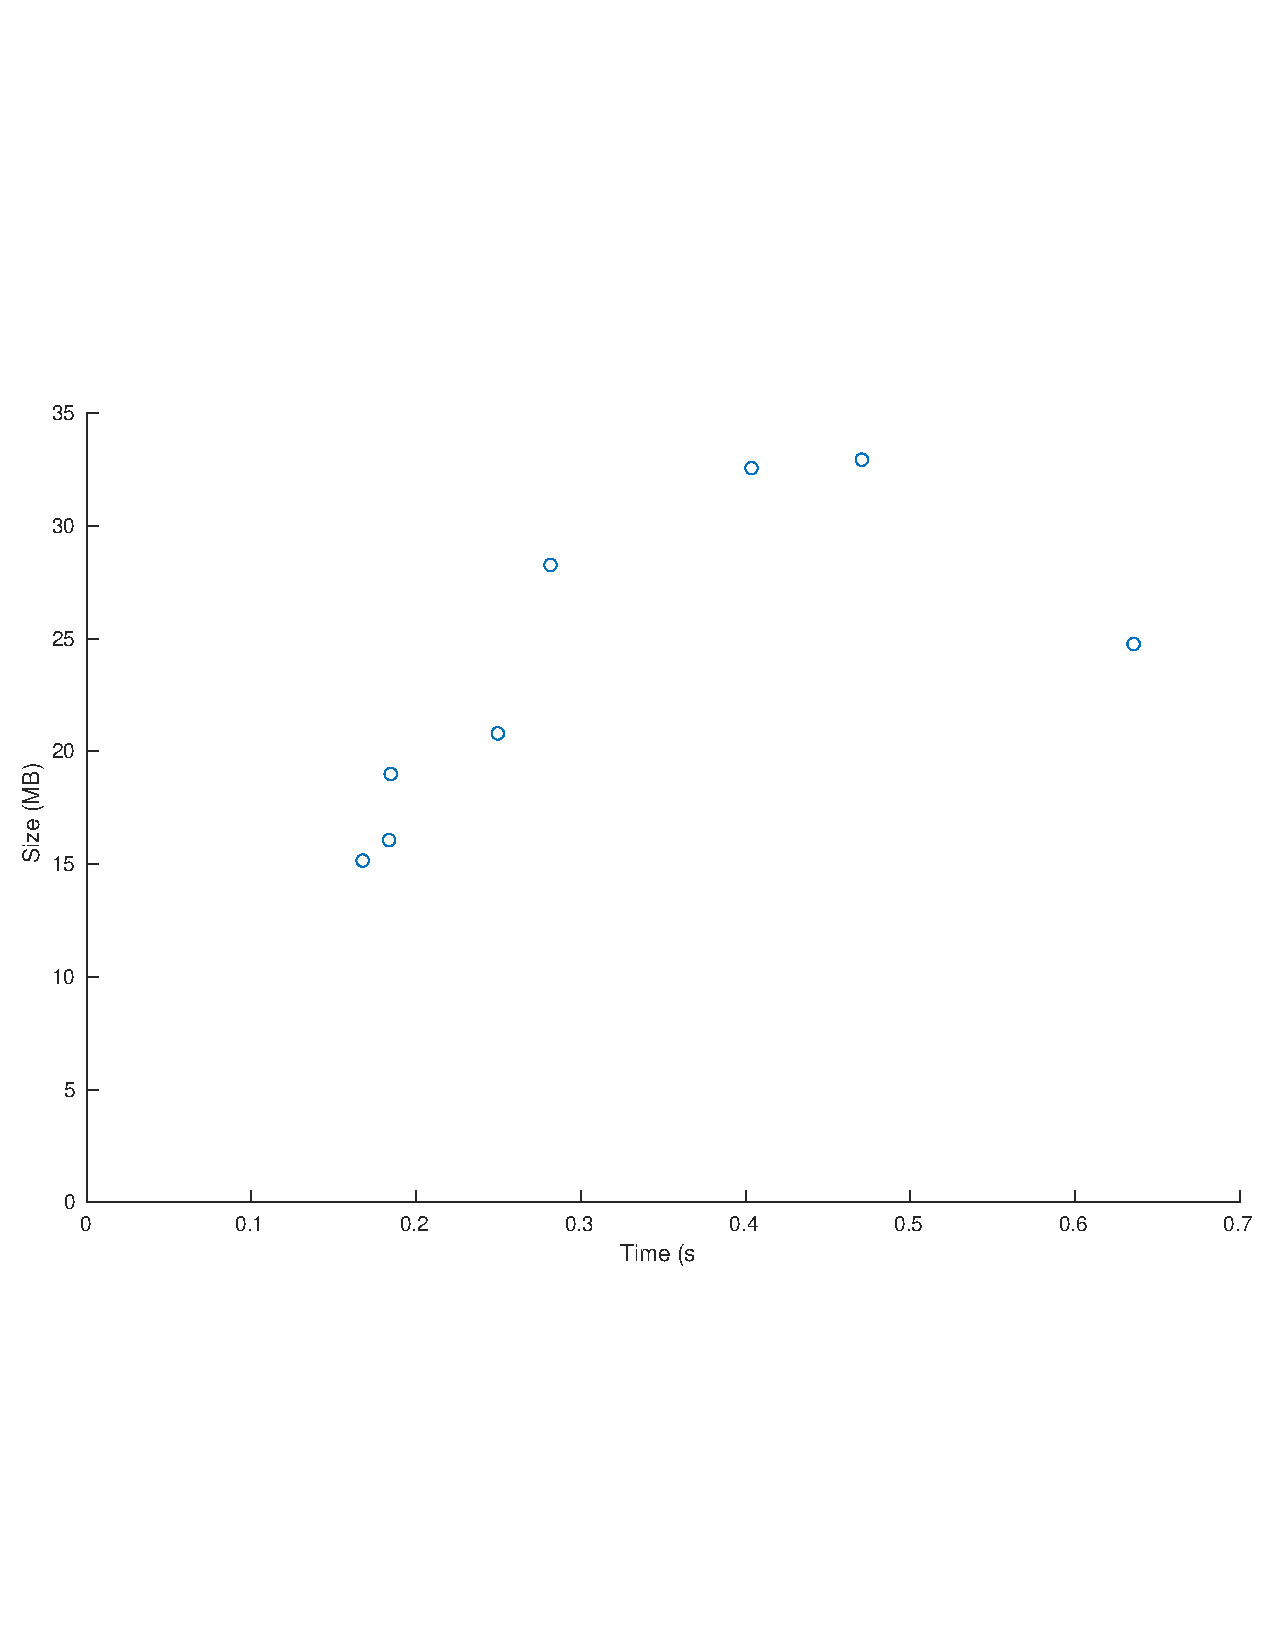
\includegraphics[trim={0cm 6.5cm 0cm 7cm},clip,width=.5\textwidth]{torrent-create-scatterplot}
	\caption{Time required to create a torrent.}
	\label{fig:torrent-create-scatterplot}
\end{figure}
% Conclusions



\section{API responsiveness}\label{sec:api_responsiveness}
% Rationale
The user expects operations to take a consistent and reasonable amount of time.
By design all functionality is going through the API.
% Metrics
connection time + latency + request processing + response processing + return latency
We use Apache JMeter to verify if the API is responding consistently within a reasonable amount of time by measuring the latency.
JMeter measures the latency from just before sending the request to just after the first response has been received. \cite{jmeter_glossary}
Thus the measurement includes the time needed to assemble the request as well as processing it and returning a response with latency on the way back.
It excludes the transfer time of the complete response and subsequent processing and rendering time.
Any client can process and render a response differently, possibly in a streaming fashion.
By leaving out that element this metric is measuring the operation time via the API.
% Expected / desired results
We want to see that the latency is bounded, consistent and generally low.
% Setup
We did the same benchmark with a slightly different setup.
A Nexus 6 smart-phone with Android 6.0.1 Cyanogen mod was connected via USB to a laptop running JMeter.
The API tcp-port was forwarded with ADB.
With JMeter we request the discovered channels from the API a 1000 times and measure the latency.
JMeter is also capable of setting a desired number of requests per minute, provided the device can handle it.
We set this parameter to 300 requests per minute, equal to the other benchmark.
% Results
The following figures show the response times for every request.
\begin{figure}[H]
	\centering
	\begin{minipage}{.49\textwidth}
		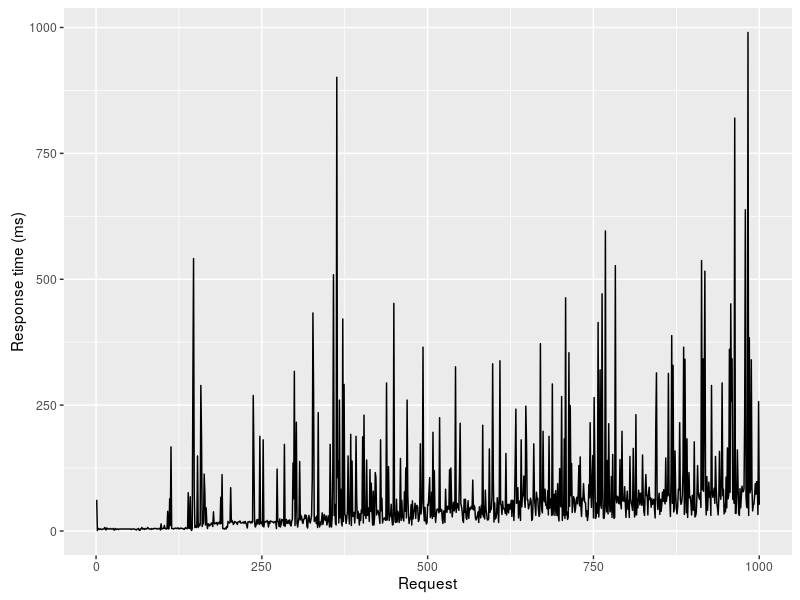
\includegraphics[width=\textwidth]{api_Laptop}
		\caption{API response times right after first launch on a decent laptop}
		\label{fig:api_Laptop}
	\end{minipage}
	~
	\begin{minipage}{.49\textwidth}
		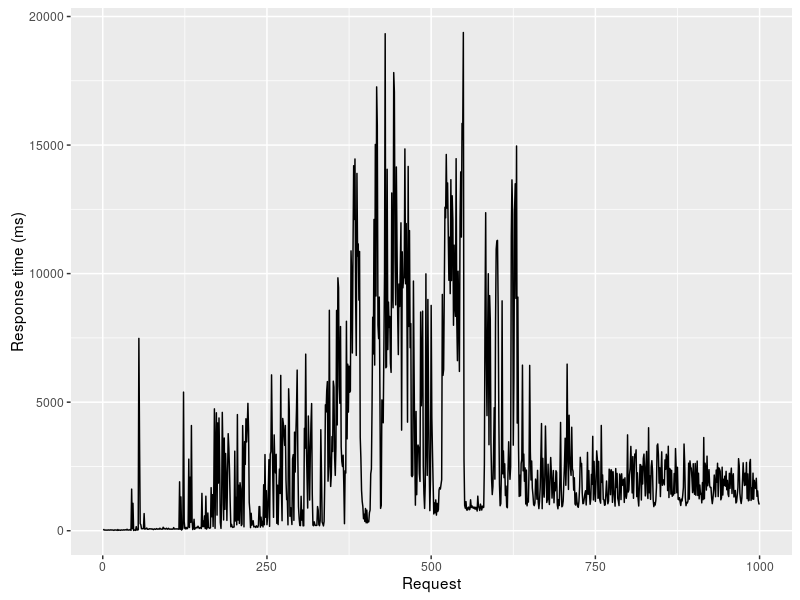
\includegraphics[width=\textwidth]{api_Nexus_6}
		\caption{API response times right after first launch on Nexus 6 smart-phone}
		\label{fig:api_Nexus_6}
	\end{minipage}
	
	\begin{minipage}{.49\textwidth}
		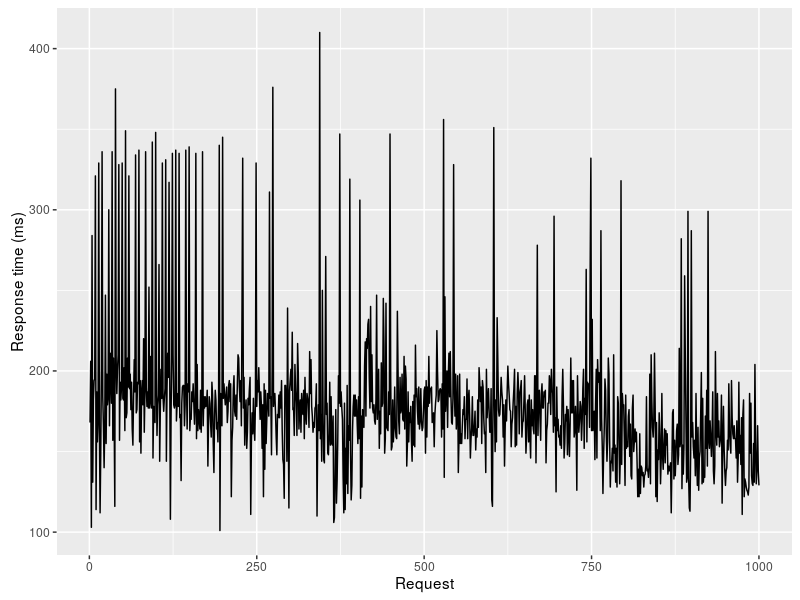
\includegraphics[width=\textwidth]{api_Laptop-2}
		\caption{API response times on a decent laptop}
		\label{fig:api_Laptop-2}
	\end{minipage}
	~
	\begin{minipage}{.49\textwidth}
		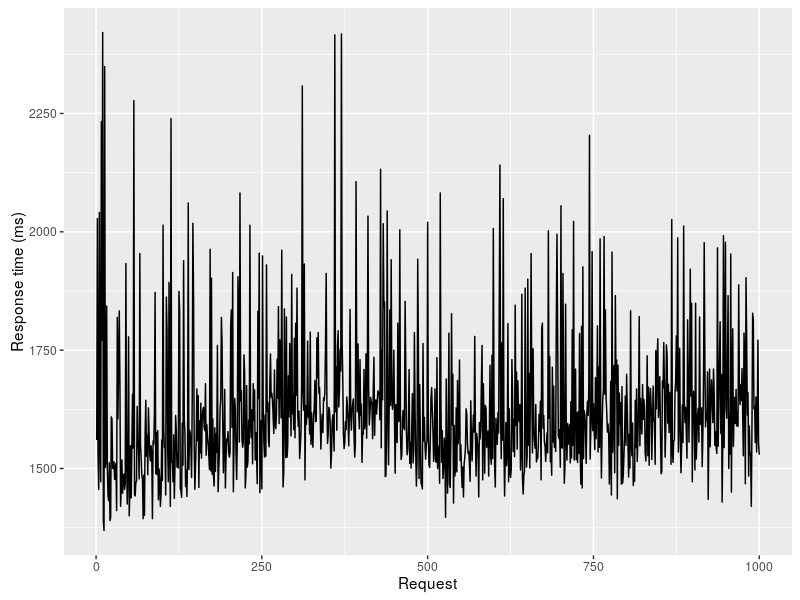
\includegraphics[width=\textwidth]{api_Nexus_6-2}
		\caption{API response times on a Nexus 6 smart-phone}
		\label{fig:api_Nexus_6-2}
	\end{minipage}
\end{figure}
The plot shows large spikes and seemingly a curious and unexpected pattern.
Table \ref{table:api_benchmark} shows the large difference in statistics.
PC is added for reference.
\begin{table}
  \begin{tabular}{l | *{8}{r}} \hline
  	 & N & Avg. (ms) & Min. (ms) & Max. (ms) & $\sigma$ (ms) & Req./min. & KB/second & Avg. Bytes \\ \hline \hline
  	 Laptop   & 1000 & 65     & 1       & 1021 & 99.00 & 60.0 & 73.72 & 75410.6 \\ \hline
  	 Nexus 6 & 1000 & 3975 & 8       & 39477 & 5362.51 & 14.4 & 49.19 & 210506.8 \\ \hline
  	 Laptop   & 1000 & 181   & 101   & 416   & 42.72   & 60.0 & 579.49 & 592791.3 \\ \hline
  	 Nexus 6 & 1000 & 1671 & 1390 & 2925 & 174.14 & 35.9 & 345.94 & 592649.8 \\ \hline
  \end{tabular}
  \caption{??}
  \label{table:api_benchmark}
\end{table}
The set rate of 300 requests per minute is clearly not reached by the smart-phone in our benchmark by a factor of 9.
The difference in amount of response data turned out to be much bigger than expected with a factor of 35.
% Conclusions
%TODO: IO bound + crappy Python code WHY?
% busy Twisted reactor?
Tribler uses the event-driven networking engine Twisted, which is also written in Python.
Twisted allows you to build inter-process communication protocols and provides a HTTP server which was used to build the REST API.
Twisted uses a single thread to coordinate all others, called the reactor thread.
If this thread is busy, the REST API can not receive incoming requests resulting in timeouts.

Considering the difference in amount of response data and the bandwidth of USB versus internal memory it is an unfair comparison.
However, based on our result we may conclude that the API does not respond consistently and appear to behave differently than the other benchmark.
The device not being able to process 5 requests per second possibly reveals information about the connection bandwidth and the multi-threaded processing capability.
We assume that the 480MB/s theoretical bandwidth of USB2.0 is not a bottleneck considering the 2,5 MB/s result of the PC.
Being a mobile device also other aspects my be at play here, like CPU frequency scaling.
However this was turned off by acquiring a wake lock from the Android OS.
It appears then that our design approach still suffers from performance issues due to imperfect multi-threaded performance.
Because if the CPU is simply not powerful enough we expect to see a linear pattern instead of what we actually see in \ref{fig:api_benchmark}.
This phenomenon is not of great importance though, because users are not expected to fire hundreds of requests per minute to the API.
Further investigation should figure out if this phenomenon is also observed with lower amounts of requests per minute.


\section{Profiling}\label{sec:profiling}
% Rationale
Because of the challenges put forward in chapter \ref{ch:tribler_mobile} we investigate if time is spent disproportionately on some function.
% Expected / desired results
We expect that the limited resources of a mobile device may impact particular features more than others.
If hardware acceleration is not present the less powerful CPU may struggle with encryption tasks.
% Metrics
Instead of CPU time, time actually spent processing by the CPU, we measure wall-clock time.
This way we measure the amount of time a user would have to wait for a certain function to be executed.
%TODO
We focus on wall clock time instead of CPU time because...

% Setup
With the cProfile Python module and the visualisation tool SnakeViz we can see if any function takes a disproportionate amount of time.
A Nexus 6 smart-phone with Android 6.0.1 Cyanogen mod was used for profiling Tribler.
The profiler was running for 10 minutes with Tribler during normal operation and without any user input.
% Results
\begin{figure}[H]
	\centering
	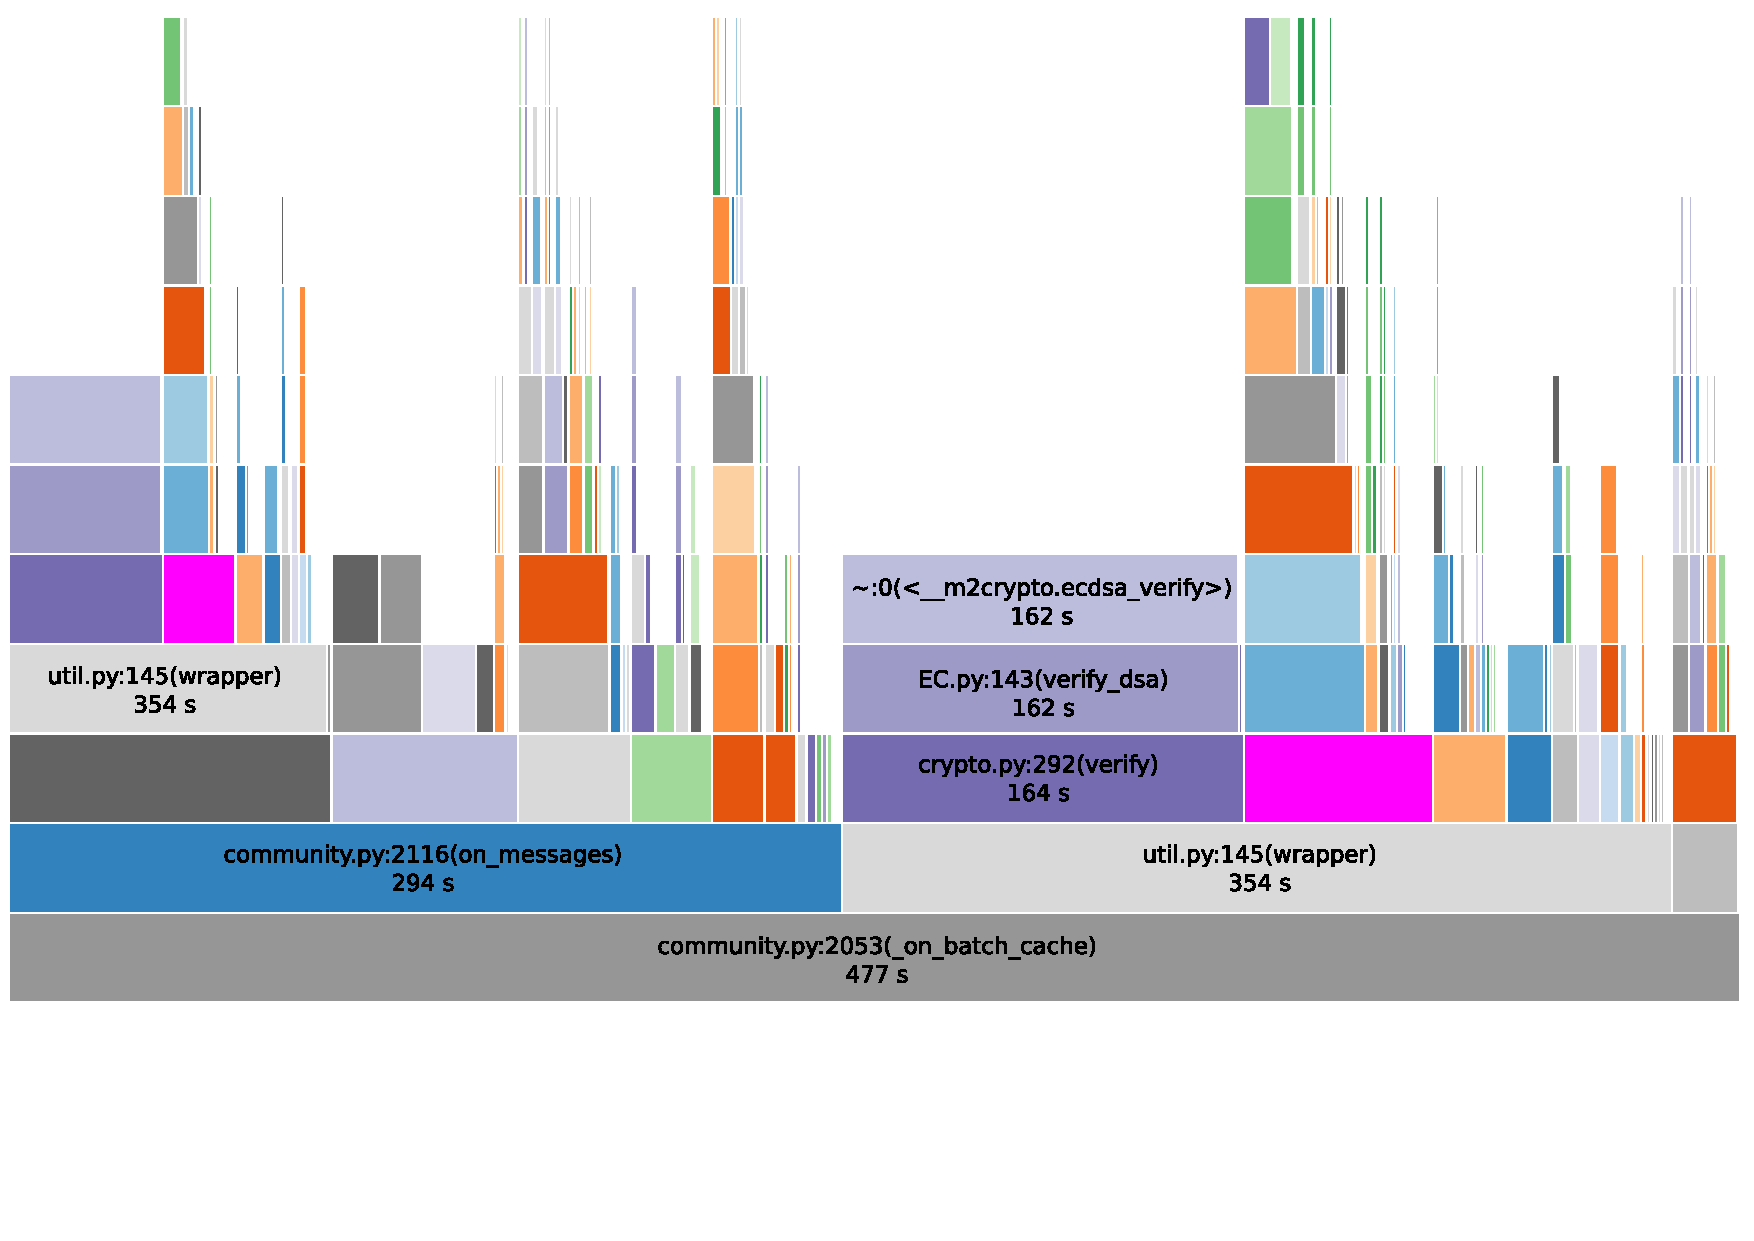
\includegraphics[width=\textwidth]{profile_1468515157-2}
	\caption{Profiler results of 10 minutes Tribler run time (bright pink represents business logic upon receiving a torrent)}
	\label{fig:profile}
\end{figure}
\begin{table}
	\begin{tabular}{*{3}{r} | l} \hline
		\# Calls & Total time (s) & Time per call (s) & Function \\ \hline \hline
		15 & 0.4867 & 0.03245 & method 'commit' of 'sqlite3.Connection' objects \\ \hline
		1 & 0.01692 & 0.01692 & method 'executescript' of 'sqlite3.Cursor' objects \\ \hline
		3820 & 64.28 & 0.01683 & method 'poll' of 'select.epoll' objects \\ \hline
		2 & 0.01048 & 0.005241 & \_\_m2crypto.ec\_key\_gen\_key \\ \hline
		31075 & 162 & 0.005212 & \_\_m2crypto.ecdsa\_verify \\ \hline
		1650 & 7.133 & 0.004323 & \_\_m2crypto.ecdsa\_sign \\ \hline
		1 & 0.001708 & 0.001708 & \_socket.gethostbyaddr \\ \hline
		1 & 0.001284 & 0.001284 & built-in method SSL\_library\_init \\ \hline
		567 & 0.565 & 0.0009965 & method 'executemany' of 'sqlite3.Cursor' objects \\ \hline
		8 & 0.005731 & 0.0009552 & \_\_import\_\_ \\ \hline
		12 & 0.01083 & 0.0009029 & method 'connect\_ex' of '\_socket.socket' objects \\ \hline
		1 & 0.00055 & 0.00055 & built-in method SSL\_load\_error\_strings \\ \hline
		5 & 0.002515 & 0.000503 & method 'recv' of '\_socket.socket' objects \\ \hline
		6989 & 3.436 & 0.0004917 & method 'executemany' of 'apsw.Cursor' objects \\ \hline
		1 & 0.000485 & 0.000485 & dir \\ \hline
		63677 & 20 & 0.000314 & method 'execute' of 'apsw.Cursor' objects \\ \hline
		5546 & 1.38 & 0.0002488 & \_\_m2crypto.ec\_key\_read\_pubkey \\ \hline
		15943 & 3.414 & 0.0002141 & method 'sendto' of '\_socket.socket' objects \\ \hline
		44 & 0.009405 & 0.0002137 & open \\ \hline
		1 & 0.000212 & 0.000212 & built-in method OpenSSL\_add\_all\_algorithms \\ \hline
		2 & 0.000405 & 0.0002025 & \_\_m2crypto.ec\_key\_new\_by\_curve\_name \\ \hline
		2 & 0.000394 & 0.000197 & netifaces.interfaces \\ \hline
		296 & 0.05179 & 0.000175 & method 'sort' of 'list' objects \\ \hline
		5 & 0.000826 & 0.0001652 & \_\_m2crypto.ec\_key\_read\_bio \\ \hline
		1 & 0.000147 & 0.000147 & \_\_m2crypto.rand\_seed \\ \hline
		4 & 0.00058 & 0.000145 & netifaces.ifaddresses \\ \hline
		47 & 0.005664 & 0.0001205 & androidembed.log \\ \hline
		12 & 0.001445 & 0.0001204 & thread.start\_new\_thread \\ \hline
		8 & 0.000936 & 0.000117 & posix.mkdir \\ \hline
		2240 & 0.2615 & 0.0001167 & posix.open \\ \hline
		17 & 0.001964 & 0.0001155 & compile \\ \hline
		3 & 0.00034 & 0.0001133 & \_\_m2crypto.ec\_key\_write\_bio\_no\_cipher \\ \hline
		5553 & 0.6196 & 0.0001116 & \_\_m2crypto.ec\_key\_write\_pubkey \\ \hline
		7 & 0.000777 & 0.000111 & method 'send' of '\_socket.socket' objects \\ \hline
		140069 & 15.4 & 0.00011 & method 'execute' of 'sqlite3.Cursor' objects \\ \hline
		16 & 0.001759 & 0.0001099 & method 'shutdown' of '\_socket.socket' objects \\ \hline
	\end{tabular}
	\caption{Native function calls wall clock time broken down per call during the 10 minute profiling (600 seconds total time)}
	\label{table:profiling_details}
\end{table}
Figure \ref{fig:profile} shows that 27\% of the time is spent on verifying cryptographic signatures.
The bright pink represents the update function, which signifies various business logic upon receiving a torrent.
Also notable is the same stack of functions within and outside of a community on top of the wrapper.
This can be explained by the fact that torrents can be discovered outside of a community too.
%TODO
execute of apsw.Cursor
execute of sqlite3.Cursor
select.epoll \cite{http://stackoverflow.com/questions/2032598/caveats-of-select-poll-vs-epoll-reactors-in-twisted}
% Conclusions
%TODO
The time per call is most important for optimization because...

The significant chunk of time that the crypto takes is as expected.
Since this task is actually delegated to the C library M2Crypto it should be possible to release the GIL of the Python interpreter so other Python code that does not depend on it can be executed.
The main alternative provided in the standard library for CPU bound applications is the multiprocessing module, which works well for workloads that consist of relatively small numbers of long running computational tasks, but results in excessive message passing overhead if the duration of individual operations is short \cite{http://python-notes.curiousefficiency.org/en/latest/python3/multicore_python.html}.
As seen from the time per call for \_\_m2crypto.ecdsa\_verify in table \ref{table:profiling_details} the multiprocessing module would likely cause too much overhead.
%TODO
Another way to optimize is multiprocessing, which avoids the GIL completely \cite{quinten}.

\section{CPU utilization}\label{sec:cpu_utilization}
%IO bound or CPU bound?
%TODO: tijdens HD streaming: net cpu over, nu nog steeds??
% let it run and measure
We saw in X that the cryptography takes a lot of time.
We need to know if this is CPU bound or not for optimization purposes.

% Rationale
Python-for-Android supplies a CPython interpreter out of the box.
CPython is optimized for single thread performance and compatibility with C extension modules.
It is limited by a global interpreter lock (GIL) in multi-threaded use cases with shared memory.
Tribler uses C extension modules for crypto tasks, which are CPU intensive.
Tribler also uses the event-driven networking engine Twisted, which is written in Python.
The core of the event loop within Twisted is the reactor, which runs on a single thread.
The reactor provides a threading interface to offload long running tasks, such as IO or CPU intensive tasks to a thread pool.
The GIL prohibits more than one thread to execute Python bytecode at a time.
This negates all performance gains in terms of parallelism afforded by multi-core CPUs, making Python threads unusable for delegating CPU bound tasks to multiple cores.
As shown in the precious section the crypto function took a considerable amount of time to compute.
To see if the releasing the GIL as put forward as a solution is feasible we measure if the CPU has more capacity than is being utilized right now.
% Metrics
During normal operation equivalent to the profiler measurement, we take a snapshot of the CPU utilization.
% Expected / desired results
If there is any performance to gain by releasing the GIL the CPU must be under-utilized right now.
% Setup
A Galaxy S3 smart-phone with Android 6.0.1 Cyanogen mod was used for this measurement.
% Results
\begin{figure}[H]
\begin{minipage}{.4\textwidth}
	\begin{adjustbox}{addcode={\begin{minipage}{\width}}{\caption{
						CPU usage on a Galaxy S3 smart-phone, about 3 hours into normal operation
			}\end{minipage}},rotate=90,center}
		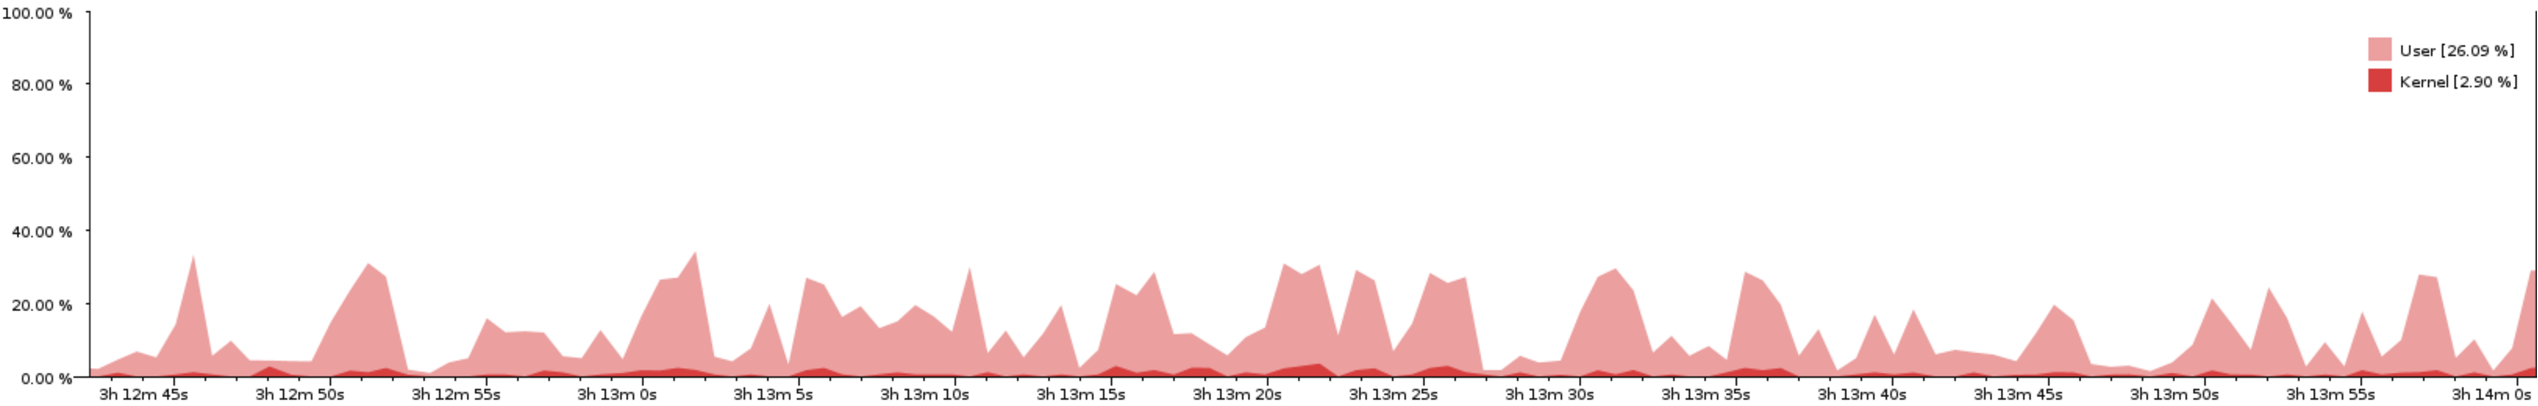
\includegraphics[scale=0.6]{monitor-cpu}
	\end{adjustbox}
	\label{fig:monitor-cpu}
\end{minipage}
~~~~~~~~~~~~~~~~~~~~
\begin{minipage}{.4\textwidth}
	\begin{adjustbox}{addcode={\begin{minipage}{\width}}{\caption{
						CPU usage on a Galaxy S3 smart-phone, about 2 minutes into the Multichain performance measurement
			}\end{minipage}},rotate=90,center}
		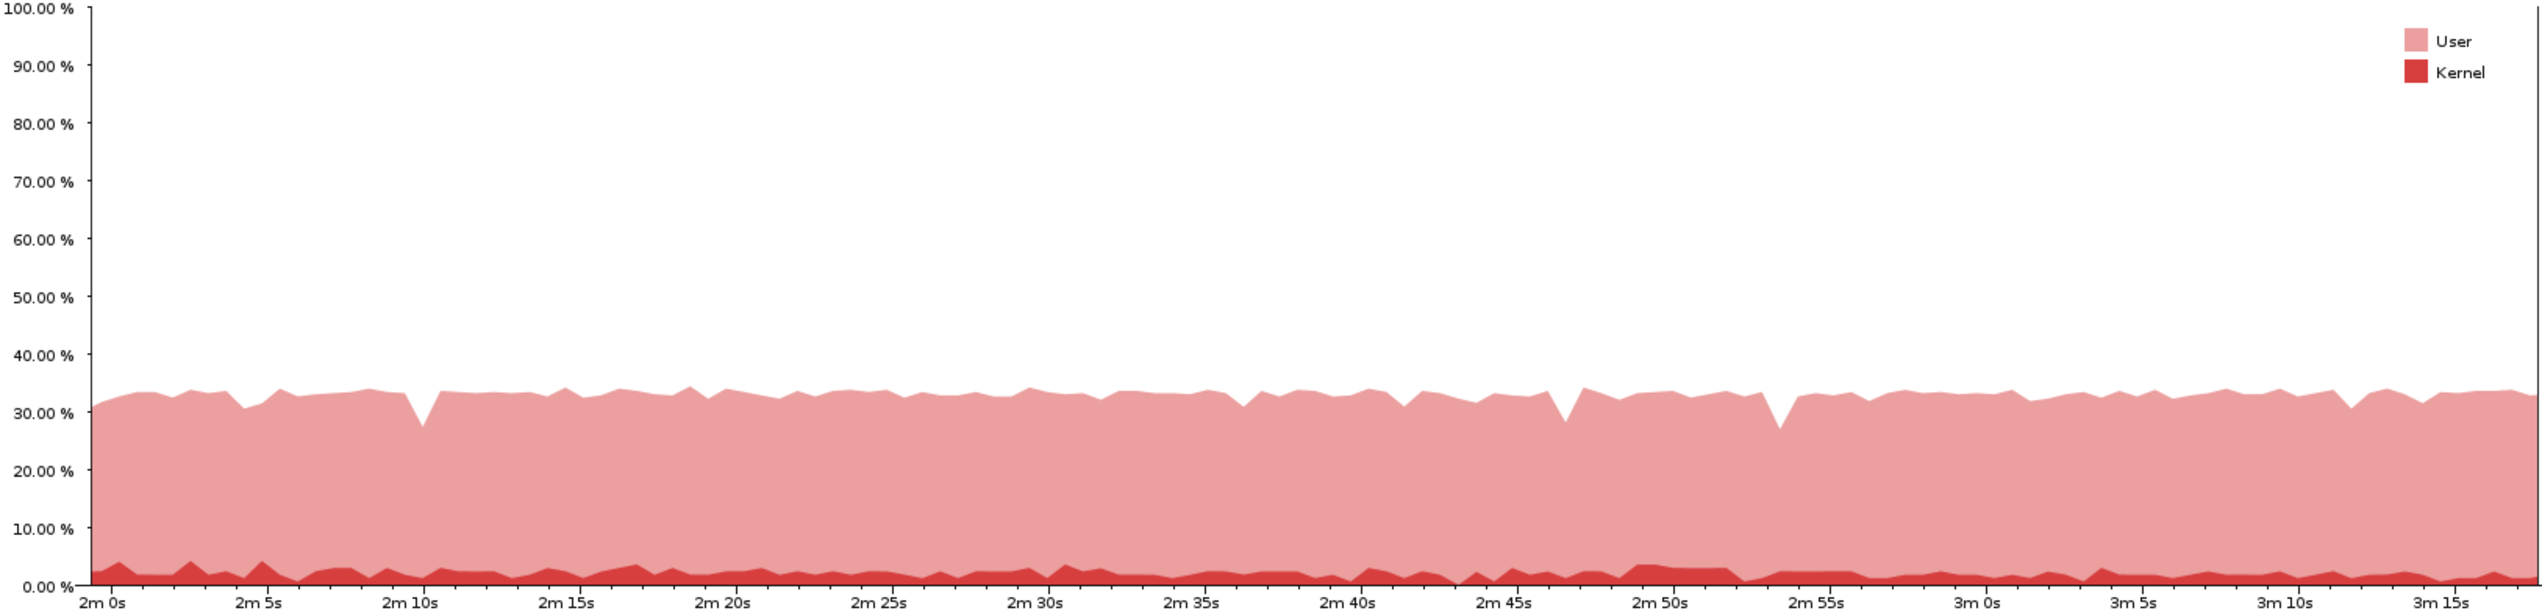
\includegraphics[scale=0.6]{monitor-cpu-experiment}
	\end{adjustbox}
	\label{fig:monitor-cpu-experiment}
\end{minipage}
\end{figure}
The results show that indeed not al 4 cores of the CPU are utilized by a large margin.
Even when performing the intensive crypto work of the Multichain experiment 2 CPU cores appear to be idling.
% Conclusions
This suggests that releasing the GIL during heavy crypto work could result in a significant performance gain.
However our results are inconclusive and warrant further research.


\section{Testing and coverage}\label{sec:testing_coverage}
% Rationale
The design choice of reusing all Tribler core source code means we need to verify its correctness.
To make sure all code on Android works the same as on other supported platforms we need to test all code.
Tribler has some unit tests and integration tests that cover a large portion of the code, but not all.
% Metrics
The ratio of tested lines of code with respect to the total number of lines of code is the coverage line-rate.
% Expected / desired results
We expect to see a line-rate value close to 1, but not 1 since we know the tests do not cover everything.
% Setup
All tests were run two times on the same device with 11 weeks of development in between.
The nose module was used for running the tests together with the coverage module for gathering coverage data.
The same Nexus 6 smart-phone with Android 6.0.1 Cyanogen mod was used in both runs.
% Results
The following table shows the results of both executions.
\begin{table}
	\begin{tabular}{l | *{5}{r}} \hline
		Run & Tests & Errors & Failures & Skipped & Line-rate \\ \hline \hline
		1     & 711   & 14       & 13          & 30          & 0.7241 \\ \hline
		2     & 749   & 12       & 15          & 3            & 0.7861 \\ \hline
		3	  & 782	  & 10		 & 18		   & 4			  & 0.7871 \\ \hline
		PC   & 812   & 0         & 0            & 30          & 0.7894 \\ \hline
		PC   & 812   & 0         & 0            & 30          & 0.7901 \\ \hline
		4     & 782   & 10       & 18          & 4            & 0.7897 \\ \hline
	\end{tabular}
	\caption{Tests results and coverage line-rate at different points in time during development}
	\label{table:testing_coverage}
\end{table}
%TODO explain failures and 30 vs 4 skipped
%GUI test fail because import Qt above @skip

The number of tests has increased as well as the coverage line-rate while the number of errors and skipped tests have decreased.
A failure means an assertion was not met and an error represents an exception while running a test.
% Conclusions
Therefore seeing that the number of failures increased is not that bad since the number of errors decreased.
If the line-rate is 1 you still need the the branch-rate to be 1 as well before you can be confident the code will work as expected.
The branch-rate is the number of code paths tested with respect to the total number of code paths possible.
Unfortunately this metric is not part of the current test plan.
Nevertheless the metrics show improvement overall.


\chapter{Conclusions and future work}
After validating and verifying our design in the previous chapter, we now come to the conclusions with regards to the main research question.

The main research question was: how feasible is it to run all Tribler functionality on mobile devices? % to defeat or mitigate large scale monitoring and censorship?

Secondary question was: given the constraints of mobile devices, what unique ability can be utilized to extend or enhance Tribler?

Secondary question was: using the unique properties of mobile devices, what features can be added or enhanced?


The feasibility in terms of functionality, performance and scalability were measured.
Several of these measurements give raise to some minor considerations.
% Profiler
The profiling revealed that crypto tasks are a significant part of processing messages.
These tasks should be offloaded to a separate computational core to release the global interpreter lock.
That would enable Python code to run in parallel, which in turn would improve performance and responsiveness.
% cpu
The CPU utilization measurement showed this approach is likely to succeed.
% Multichain
The Multichain measurement showed that database performance in that instance was stringent in the current implementation.
It is also the most easy to resolve by keeping the hash of the last block for connected peers in memory .
% Tests
All existing tests can be run on Android just as well as on other platforms.
This means, in combination with the modularity of the new design and re-use of the Tribler core, that maintainability and testability are very fit.
% Startup
In terms of user experience the measurement of startup time showed to be very consistent and reasonable.
% Latency
The latency of the API however seemingly showed a curious pattern that cannot be explained right away.
It is only known to occur if hundreds of requests per minute are fired at the API, which is unexpected behavior from the user.

Finally, to answer the secondary question: using the unique properties of mobile devices, what features can be added or enhanced?
% Bluetooth
We added the capability to transfer the app to another device that doesn't have it yet via Bluetooth.
% nfc
If NFC is enabled on both devices the app can be transfered by just holding the devices next to each other.
Also adding a channel to your favorites can be done this way.
Using your real life social network you can build your on-line trusted network this way.
% P2P Wifi
And thanks to built-in hardware capability you can setup an ad hoc WiFi network to avoid any infrastructure completely.


What this means in the context of privacy and censorship is that if content is detected by the censor it may have already crossed or will cross the freedom border thanks to the properties of viral spreading.




% Research Limitations
% Project scope
% broad / narrow scope, scope of other system()s)
% sub-problems
% ultimate high-level goal
Software development / technical aspect only
Not policy making, organisational perspective, decision making, normative, ethical,
Time limit of 9 months


%% Use letters for the chapter numbers of the appendices.
\appendix

%\input{appendix-a}

\bibliography{thesis}
	
\end{document}
